\documentclass[conference]{IEEEtran}
\IEEEoverridecommandlockouts
% The preceding line is only needed to identify funding in the first footnote. If that is unneeded, please comment it out.
\usepackage{cite}
\usepackage{amsmath,amssymb,amsfonts}
\usepackage{algorithmic}
\usepackage{graphicx}
\usepackage{textcomp}
\usepackage{xcolor}
\usepackage{booktabs}
\usepackage{array}
\usepackage{multirow}
\usepackage{url}
\usepackage{eurosym}
\usepackage{textcomp}
\usepackage{hyperref}

\def\BibTeX{{\rm B\kern-.05em{\sc i\kern-.025em b}\kern-.08em
    T\kern-.1667em\lower.7ex\hbox{E}\kern-.125emX}}
    
% ===================== ADDED THIS =====================

\renewcommand{\thesection}{\arabic{section}}
\renewcommand{\thesubsection}{\thesection.\arabic{subsection}}
\renewcommand{\thesubsectiondis}{\thesubsection}

% =====================================================

\begin{document}

\title{Deep Learning for Panoramic Dental Radiographs: A Comprehensive
Survey on Caries Detection, Periodontal Bone Loss Assessment and
Explainable AI%

}

\author{
\IEEEauthorblockN{C S Deepak}
\IEEEauthorblockA{\textit{Dept.\ of Computer Science}\\
\textit{PES University -- RR Campus}\\
Bangalore, India}
\and
\IEEEauthorblockN{Chennupati Gunadeep}
\IEEEauthorblockA{\textit{Dept.\ of Computer Science}\\
\textit{PES University -- RR Campus}\\
Bangalore, India}
\and
\IEEEauthorblockN{Archana}
\IEEEauthorblockA{\textit{Dept.\ of Computer Science}\\
\textit{PES University -- RR Campus}\\
Bangalore, India}
\and
\IEEEauthorblockN{AVSN Sai Srujan}
\IEEEauthorblockA{\textit{Dept.\ of Computer Science}\\
\textit{PES University -- RR Campus}\\
Bangalore, India}
\and
\IEEEauthorblockN{\centering Under the guidance of Dr.\ Mamatha H R, Director, Bajaj Engineering Skills Training @PESU, Bangalore, India}
}
\maketitle

% -----------------------------------------------------------------------
\begin{abstract}
Dental panoramic radiographs (OPGs) are the primary clinical tool for
diagnosing caries and periodontal disease, yet manual interpretation is
slow and varies substantially between examiners. Deep learning has
advanced considerably, but most published systems address a single
diagnostic task in isolation, leaving the clinical integration problem
unsolved.

This paper surveys 70 deep learning studies published between 2021 and
2026, covering caries detection, severity staging, periodontal bone loss
assessment, tooth segmentation, and explainable AI. Architectures
examined include CNNs, YOLO-based detectors, U-Net variants,
transformer-based models, and, most recently, vision-language models.
We formally define a unified multi-task dental AI framework that
combines detection, localization, severity staging, quantification, and
explainability within a single system.

Most studies address individual sub-tasks well, and a small number of
very recent large-scale vision-language systems trained on proprietary
multi-hospital data now integrate detection, tooth numbering, and
free-text report generation into one deployed pipeline. However, no
publicly reproducible system (open in both model weights and training
data) combines detection, quantitative severity staging, and
periodontal bone-loss measurement within a single panoramic-radiograph
pipeline. Five recurring gaps are identified: task fragmentation across
the openly reproducible literature, absent severity staging, low
explainability adoption, dataset bias, and limited clinical
integration.

The analysis provides a structured foundation for building the next
generation of clinically deployable dental AI systems.
\end{abstract}

\begin{IEEEkeywords}
Deep Learning, Dental Caries, Periodontal Disease, Panoramic
Radiographs, Tooth Segmentation and Detection, Multi-Task Learning,
Explainable AI
\end{IEEEkeywords}

% -----------------------------------------------------------------------
\section{Introduction}
\label{sec:intro}

Dental panoramic radiography, also known as OrthoPantomography (OPG),
is the standard imaging tool in routine dental practice. A single
panoramic exposure captures the full dentition, surrounding alveolar
bone, and anatomical landmarks in one image, making it the primary
modality for detecting dental caries, periodontal bone loss, impacted
teeth, and other oral pathologies. Accurate interpretation nevertheless
requires substantial expertise and is subject to inter-examiner
variability, a problem that affects early-stage practitioners such as
dental students and interns more acutely than experienced clinicians.

Dental caries, defined as the progressive bacterial demineralization of
tooth enamel and dentine, affects approximately 2.3 billion people
globally and is the most prevalent non-communicable disease worldwide
\cite{luke2025accuracy}. Periodontal disease, characterized by
irreversible alveolar bone loss around the teeth, affects over 19\% of
the adult global population and is the leading cause of adult tooth
loss \cite{khubrani2025detection}. Both conditions share a clinically
consequential property: their early radiographic signs are subtle and
easily missed. A faint radiolucency at the proximal surface of a
premolar, or a 1--2\,mm reduction in alveolar bone height, can alter
the clinical decision yet remain visually ambiguous even for trained
examiners.

Over the past five years, deep learning has produced notable gains in
automated dental radiograph analysis. Convolutional neural networks
(CNNs), YOLO-based object detectors, U-Net segmentation architectures,
and transformer-based models have demonstrated competitive performance
across individual diagnostic tasks such as caries detection, tooth
segmentation, and periodontal bone loss estimation
\cite{nassiri2025yolo,jundaeng2025advanced,bhoopalan2026self}.

These advances have not, however, resolved the fragmentation that
characterizes the field at the system level. Most published approaches
target isolated tasks or single-disease objectives; the components
required for a complete clinical workflow are rarely combined. The
underlying problem is structural: models are tuned for task-specific
metrics rather than the kind of holistic diagnostic reasoning that
clinical use demands \cite{zanini2024systematic,muresanu2024automating}.

Automated dental radiograph analysis is multi-dimensional by nature. A
clinically viable system must handle multi-instance detection across all
teeth, identify low-contrast early-stage lesions, measure anatomical
landmarks such as the cemento-enamel junction (CEJ) and alveolar bone
crest, and manage the co-occurrence of multiple diseases within a single
panoramic image. This diagnostic process can be
conceptualized as a pipeline, as illustrated in Fig.~\ref{fig:pipeline}.

\begin{figure*}[tp]
    \centering
    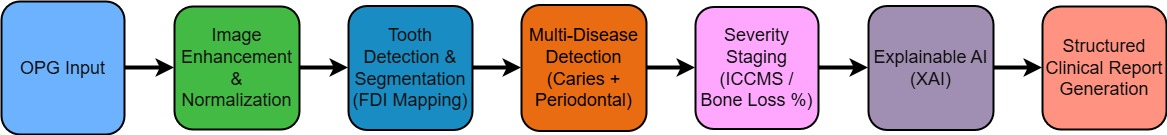
\includegraphics[width=\textwidth]{fig1.jpeg}
    \caption{System Pipeline of Proposed AI Model.}
    \label{fig:pipeline}
\end{figure*}

The absence of standardized datasets and evaluation protocols further
limits reproducibility and cross-study comparability. A large proportion
of studies rely on private, single-center data, which introduces dataset
bias and reduces generalization to external clinical environments
\cite{muresanu2024automating,delamare2024panoramic}. Explainable AI
(XAI) is also rarely implemented, despite its recognized role in
building clinical trust, supporting regulatory acceptance, and enabling
interpretable output \cite{ferrara2025applications,bilal2024pdcnet}.
Without explainability, combined with inconsistent validation practices,
clinical deployment remains out of reach for most published systems.

Rather than surveying individual tasks or model architectures in
isolation, this work takes a system-level perspective, examining how
individual components might be combined into a unified diagnostic
framework \cite{zhou2025deep,albano2024artificial}.

The survey covers 70 papers published between 2021 and 2026, organized
into six functional categories: caries detection and severity
classification, periodontal disease and bone loss analysis, multi-task
end-to-end diagnosis, explainable AI, dataset benchmarking and clinical
validation, and tooth segmentation and numbering. The central finding is
narrower than it would have been eighteen months ago: a small number of
2026 vision-language systems, most notably DentFound
\cite{zhu2026dentfound}, now combine tooth detection, FDI numbering,
caries and periodontal findings, post-hoc explainability, and free-text
report generation in one deployed system validated on over 101,000
patients. What no reviewed system provides -- DentFound included -- is
a \emph{publicly reproducible} pipeline (open model weights and open
training data) that also performs quantitative severity staging and
periodontal bone-loss measurement rather than qualitative narrative
findings. The unmet need this survey establishes is therefore
reproducibility and measurement granularity within an integrated
pipeline, not the mere existence of an integrated pipeline.

The main contributions of this survey are as follows:
\begin{itemize}
    \item A task-level taxonomy of deep learning systems for panoramic
          dental radiograph analysis, covering detection, segmentation,
          classification, and multi-task architectures.
    \item A formal problem formulation for unified multi-disease dental
          diagnosis, highlighting the integration requirements of
          detection, severity staging, quantification, and
          explainability.
    \item A cross-category comparative analysis of 70 studies,
          identifying inconsistencies in datasets, evaluation metrics,
          and validation protocols.
    \item A quantified gap analysis revealing key limitations in current
          research, including single-disease model focus, absence of
          automated severity staging, dataset fragmentation, and low
          adoption of explainable AI.
    \item A research roadmap toward clinically deployable, explainable,
          multi-task dental AI systems.
\end{itemize}

A unified, explainable, multi-task approach to dental AI is the logical
next step toward systems that can be deployed in clinical practice,
particularly for supporting junior clinicians and dental students.




% -----------------------------------------------------------------------
\section{Search Methodology}
\label{sec:methodology}

This survey used a structured keyword search across five digital
libraries: IEEE Xplore, PubMed/MEDLINE, Scopus, Google Scholar, and
SpringerLink, restricted to papers published from 2020 onward. The
search was conducted in three rounds: an initial search between
January and December 2024; a first update extending coverage to March
2025; and a final update, focused on arXiv, Nature Portfolio, MDPI, and
NeurIPS/MICCAI proceedings venues, conducted in August 2026 to capture
the most recent vision-language and benchmark systems before
submission. All results reported in this survey reflect the corpus as
of the August 2026 update.

\subsection{Search Strategy}

Search queries were organized into five thematic clusters:

\begin{itemize}
  \item \textit{Caries detection on panoramic radiographs:}
        ``dental caries'' panoramic radiograph deep learning; ``caries
        detection'' panoramic radiograph CNN; ``caries segmentation''
        orthopantomogram neural network.

  \item \textit{Periodontal disease and bone loss:} ``periodontal
        disease'' panoramic radiograph deep learning; ``alveolar bone
        loss'' orthopantomogram AI; ``CEJ'' ``bone crest'' panoramic
        radiograph segmentation.

  \item \textit{Multi-disease and end-to-end OPG systems:}
        ``multi-task'' dental panoramic radiograph deep learning;
        ``dental disease detection'' panoramic radiograph end-to-end.

  \item \textit{Explainable AI in dental imaging:} ``explainable AI''
        dental radiograph; ``Grad-CAM'' dental panoramic;
        ``interpretable deep learning'' dental imaging.

  \item \textit{Dataset and clinical validation:} ``dental panoramic
        radiograph dataset'' deep learning; ``OPG benchmark'' AI;
        ``clinical validation'' dental AI panoramic.
\end{itemize}

\subsection{Inclusion and Exclusion Criteria}

Papers were included if they: (i)~applied deep learning or machine
learning to dental radiograph analysis; (ii)~used panoramic, bitewing,
or periapical radiographs as primary input; (iii)~targeted detection,
segmentation, classification, or staging of dental caries, periodontal
disease, or related pathologies; and (iv)~reported quantitative
performance metrics. Papers were excluded if they focused exclusively on
CBCT/3D imaging, addressed only non-dental imaging, or did not report
reproducible quantitative results. Clinical reviews without AI models
were included only when they provided foundational clinical definitions
directly relevant to the survey scope.

\subsection{Final Corpus}

After applying the criteria, 70~papers were selected, spanning
2021--2026: 19~from 2026 (27.1\%), 31~from 2025 (44.3\%), 17~from 2024
(24.3\%), 2~from 2023 (2.9\%), and 1~from 2021 (1.4\%). This
distribution reflects the field's rapid growth over recent years, and
in particular a sharp acceleration in 2026 driven largely by
vision-language and multimodal-benchmark systems. Of the original
47-paper base corpus (collected through March 2025), publication
venues included BMC Oral Health (8~papers), IEEE (8), MDPI journals
(9), Elsevier (4), Springer (3), and Scientific Reports/Nature
Portfolio (3). The 23~papers added in the August 2026 update skew
further toward Nature Portfolio journals (5, including Scientific
Reports, \emph{Nature Biomedical Engineering}, npj Digital Medicine,
and Scientific Data), MDPI journals (5), and arXiv preprints (5),
reflecting how quickly large vision-language and benchmark work in
this space is currently moving to preprint servers ahead of peer
review.

% -----------------------------------------------------------------------
\section{System-Level Taxonomy and Problem Formulation}
\label{sec:taxonomy}

\subsection{Formal Problem Definition}

Panoramic dental radiograph analysis is a multi-component diagnostic
problem that cannot be reduced to single-task prediction.
In clinical practice, meaningful diagnosis requires coordinated
execution of several interdependent processes: localization of teeth,
identification of pathological conditions, assessment of disease
severity, and quantitative measurement of relevant anatomical
parameters. Most deep learning systems in the reviewed
literature address only one of these components
\cite{albano2024artificial,luke2025accuracy,zanini2024systematic},
producing outputs that are diagnostically incomplete and difficult to
use in a clinical setting.

A unified dental AI system maps an input OPG to structured diagnostic
outputs through six core functional components: detection, localization,
severity staging, quantification, explainability, and clinical
integration. To our knowledge, no reviewed study in the
corpus of 70 papers fully addresses all six components simultaneously
\emph{and} reproducibly on panoramic radiographs -- the closest
approach, DentFound \cite{zhu2026dentfound}, covers detection,
localization, explainability, and clinical integration but not
quantitative severity staging or bone-loss measurement, and releases
neither its weights nor its training data. That gap is the primary
motivation for this survey.

These six core components are defined as follows:

\begin{itemize}
    \item \textbf{Detection:} Identification of pathological conditions
          from radiographic features (carious lesions, periodontal bone
          loss, periapical pathology, impacted teeth). YOLO-family
          architectures dominate this task
          \cite{ayhan2025detection,nassiri2025yolo,chen2024cariesxrays,
          bizjak2024advancing,pornprasertsuk2025clinical}.

    \item \textbf{Localization:} Spatial identification of affected
          teeth through bounding boxes or polygon segmentation.
          Tooth-level localization using FDI numbering is present in
          pipeline systems
          \cite{jundaeng2025advanced,chen2024cariesxrays,bizjak2024advancing,
          pornprasertsuk2025clinical} but absent in
          classification-only approaches
          \cite{kaushik2025densenet201,mathur2025comparative,ozdemir2026enhanced}.

    \item \textbf{Severity Staging:} Classification of disease
          progression along clinically meaningful scales. For caries:
          enamel, dentine, pulp involvement
          \cite{asadi2024detection,bizjak2024advancing}. For
          periodontal disease: Stages I--IV per 2018 AAP/EFP
          classification \cite{chmielewski20252018}. This remains a
          critically underaddressed component: three C1 papers now
          provide caries severity differentiation
          \cite{bizjak2024advancing,asadi2024detection,wang2026transformer},
          led by Wang and Li's D1--D4 staging transformer
          \cite{wang2026transformer}, and two C2 systems now stage
          periodontal severity on panoramic-adjacent data
          \cite{le2026automated,li2025novel} -- neither yet mapped
          explicitly onto the 2018 AAP/EFP Stage I--IV taxonomy used in
          this survey.

    \item \textbf{Quantification:} Measurement of the CEJ--alveolar
          bone crest distance and percentage bone loss. Four studies
          address this: Jundaeng et al.\ achieved
          mAP50\,=\,0.995 \cite{jundaeng2025advanced}; Wimalasiri et
          al.\ reported ICC\,=\,0.80 \cite{wimalasiri2025ai}; Tian
          et al.\ achieved ICC\,=\,0.83 \cite{tian2025development}; and
          Le et al.\ reported per-tooth-type PCC/ICC agreement for
          radiographic bone loss from a six-keypoint pipeline
          \cite{le2026automated}, the most granular quantification
          result in the corpus.

    \item \textbf{Explainability:} Generation of interpretable visual
          outputs for clinical verification. 9 of 70 papers now
          implement some form of explainability (12.9\%, up from 6.4\%
          in the pre-2026 corpus): Chen et al.\
          \cite{chen2023deep} and Bilal et al.\ \cite{bilal2024pdcnet}
          use Grad-CAM, Chen et al.\ \cite{chen2024cariesxrays} and
          Wang and Li \cite{wang2026transformer} show feature/attention
          map visualization, and DentFound, George et al., Ren and
          Chen, Alnasser et al., and Li et al.\ add Grad-CAM,
          XGrad-CAM, or CAM-based explanations to 2025--2026 systems
          \cite{zhu2026dentfound,george2026explainable,ren2026dualbranch,alnasser2026advanced,li2025novel}.

    \item \textbf{Clinical Integration:} Alignment with diagnostic
          workflows, reporting standards, and regulatory requirements.
          Only Schwendicke et al.\ \cite{schwendicke2021cost} model
          economic impact, and only Lee et al.\ \cite{lee2025evaluation}
          measure clinician acceptance through a 65-dentist usability
          survey.
\end{itemize}

This six-component formulation stands in direct contrast to existing
approaches that address each task in isolation -- a fragmentation
independently identified as critical by multiple systematic reviews
\cite{iacob2025automated,albano2024artificial,bonfanti2025deep,
khubrani2025detection,zanini2024systematic,zhou2025deep}.

\subsection{System Taxonomy}

Existing approaches can be categorized into four distinct system
archetypes based on task integration and diagnostic scope. This taxonomy
reveals both progression toward integration and persistent limitations
preventing full clinical utility. Table~\ref{tab:taxonomy} summarizes
capability coverage across taxonomy dimensions.

\subsubsection{Single-Task Approaches}

Single-task systems address one diagnostic objective in isolation --
caries detection, tooth segmentation, or periodontal classification --
without integration. This accounts for the majority of reviewed studies
(21 C1, 18 C2 papers). While several achieve high performance --
CariesXrays FPCL reaching AP50\,=\,84.1\% \cite{chen2024cariesxrays},
Attention U-Net achieving Recall\,=\,0.96
\cite{pornprasertsuk2025clinical}, U-Net variants reporting
Dice\,=\,96.77\% \cite{vickram2025extraction} -- none produce severity
grading, periodontal assessment, or clinical explanations. The
fundamental limitation is not performance but scope: optimizing one
component without modeling interdependence with other diagnostic tasks
produces clinically incomplete systems. Systematic reviews confirm this
\cite{albano2024artificial,zanini2024systematic}, identifying absence
of multi-task integration as the primary barrier to clinical
translation.

\subsubsection{Multi-Task Approaches}

Fourteen reviewed papers adopt multi-task designs with varying
completeness, seven of them added in the August 2026 update
(Section~\ref{sec:multitask}). Chen et al.\ \cite{chen2023deep} is the most clinically
complete, classifying both periodontitis and caries on a per-tooth
basis using EfficientNet-B0 with YOLOv7 localization (ROC
AUC\,=\,98.67\% for periodontitis, 98.31\% for caries) with Grad-CAM
explainability. However, this system operates exclusively on periapical
radiographs -- not panoramic OPGs -- limiting direct applicability.
Multi-task approaches expose a critical performance asymmetry:
structural tasks (segmentation, enumeration) consistently achieve
near-ceiling performance, while pathological tasks (disease detection,
severity staging) remain substantially harder. Mure\c{s}anu et al.\
\cite{muresanu2024automating} quantified the real-world cost: YOLOv8
F1 dropped from 0.60 (internal) to 0.47 (external) -- a 22\%
degradation from single-center training.

\subsubsection{Pipeline-Based Approaches}

Pipeline systems decompose diagnosis into sequential stages, reflecting
the staged clinical reasoning dentists employ. Jundaeng et al.\
\cite{jundaeng2025advanced} implemented a precise periodontal pipeline:
YOLOv8 Stage~1 for tooth segmentation (mAP50\,=\,0.92) feeds Stage~2
for CEJ and bone crest detection (mAP50\,=\,0.995,
Sensitivity\,=\,1.0). Pornprasertsuk-Damrongsri et al.\
\cite{pornprasertsuk2025clinical} combined YOLOv5s for tooth detection
with Attention U-Net for caries segmentation (Recall\,=\,0.96,
F1\,=\,0.85). The inherent limitation is error propagation:
inaccuracies in early stages compound through subsequent stages. None
of the reviewed pipelines address severity staging, and explainability
appears in only one system \cite{chen2023deep} -- operating on
periapical, not panoramic, radiographs.

\subsubsection{End-to-End Approaches}

End-to-end models directly map radiographs to diagnostic outputs using
deep architectures -- primarily transformers. Bhoopalan et al.\
\cite{bhoopalan2026self} applied Vision Transformer and Swin Transformer
to 5,098 OPGs, achieving ViT accuracy\,=\,96\% without spatial
localization or severity grading. Van Nistelrooij et al.\
\cite{vannistelrooij2024combining} combined Mask DINO with Swin-B
Transformer, achieving tooth-level assessment performance
(FROC\,=\,0.988) but with 40-second inference time unsuitable for
clinical use. The fundamental barrier has long been data: the field
lacked large-scale, multi-disease, multi-center datasets required for
end-to-end learning. DentFound~\cite{zhu2026dentfound} shows this
barrier is surmountable given sufficient (private) institutional data
-- over 101,000 patients across four centers -- while
MMOral~\cite{hao2025mmoral} shows a public dataset at meaningful scale
(20,563 radiographs) is now available, though not yet paired with an
open, end-to-end trained model of DentFound's scope.

The system-level taxonomy and capability gaps across different architectural paradigms are illustrated in Fig.~\ref{fig:taxonomy}

\begin{figure*}[t]
  \centering
  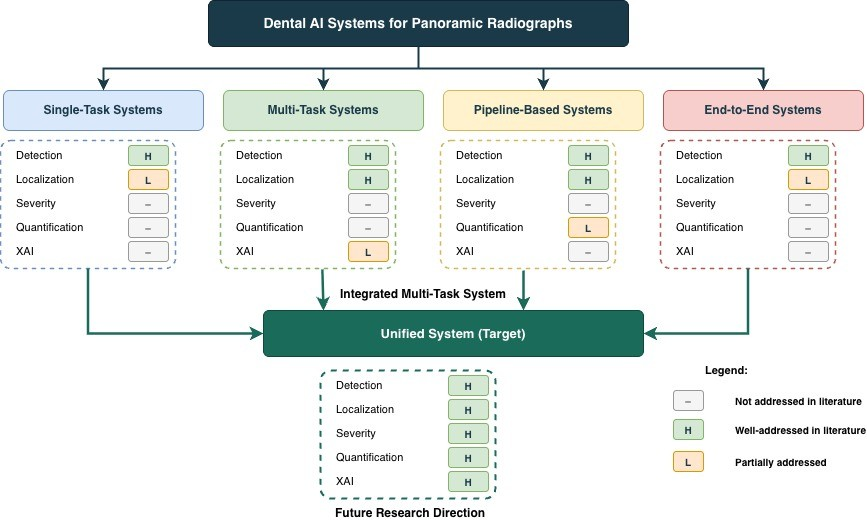
\includegraphics[width=0.85\textwidth]{fig4.jpeg}
  \caption{System-level taxonomy of dental AI approaches for panoramic radiographs, 
  illustrating four architectural paradigms (Single-Task, Multi-Task, Pipeline-Based, 
  and End-to-End Systems) and their respective capability coverage across detection, 
  localization, severity, quantification, and explainability (XAI) dimensions, 
  alongside the proposed Unified System as a future research direction.}
  \label{fig:taxonomy}
\end{figure*}

\begin{table*}[t]
\renewcommand{\arraystretch}{1.5}
\caption{System Taxonomy --- Representative Studies by Design Pattern
and Capability Coverage}
\label{tab:taxonomy}
\centering
\scriptsize
\setlength{\tabcolsep}{4pt}
\begin{tabular}{p{1.6cm} p{3.5cm} p{1.0cm} p{1.2cm} p{1.2cm} p{1.0cm} p{1.0cm} p{1.5cm}}
\toprule
\textbf{System Type} & \textbf{Representative Studies} &
\textbf{Detect} & \textbf{Localize} & \textbf{Severity} &
\textbf{Quant.} & \textbf{XAI} & \textbf{Multi-Disease} \\
\midrule
Single-Task &
\cite{ayhan2025detection,alharbi2023detection,khuwaja2024ai,
chen2024cariesxrays,perez2024ai,zancan2025ai,ozdemir2026enhanced}
& \checkmark & Partial & \texttimes & \texttimes & \texttimes & \texttimes \\

Multi-Task &
\cite{nassiri2025yolo,chen2023deep,gamal2025automated,
vannistelrooij2024combining,muresanu2024automating,bhoopalan2026self}
& \checkmark & \checkmark & \texttimes & \texttimes & Partial & Partial \\

Pipeline-Based &
\cite{jundaeng2025advanced,chen2024cariesxrays,bizjak2024advancing,
pornprasertsuk2025clinical}
& \checkmark & \checkmark & \texttimes & Partial & \texttimes & \texttimes \\

End-to-End &
\cite{vannistelrooij2024combining,bhoopalan2026self}
& \checkmark & Partial & \texttimes & \texttimes & \texttimes & Partial \\

Vision-Language (2026) &
\cite{zhu2026dentfound}
& \checkmark & \checkmark & \texttimes & \texttimes & Partial & \checkmark \\

\midrule
\textbf{Unified (Required)} & \textit{None openly reproducible in reviewed corpus}
& \checkmark & \checkmark & \checkmark & \checkmark & \checkmark & \checkmark \\
\bottomrule
\multicolumn{8}{l}{\footnotesize \checkmark\,=\,fully addressed;\
\texttimes\,=\,not addressed;\ Partial\,=\,partially addressed.}\\
\multicolumn{8}{l}{\footnotesize Quant.\,=\,quantitative measurement;\
XAI\,=\,explainable AI outputs.}\\
\multicolumn{8}{l}{\footnotesize DentFound integrates 4 of 6 dimensions but lacks severity/quantification and open weights/data.}\\
\end{tabular}
\end{table*}

\subsection{Task Hierarchy}

Dental radiograph analysis follows a structured sequence of
interdependent processing stages reflecting the actual cognitive process
trained clinicians employ:

\begin{figure*}[t]
  \centering
  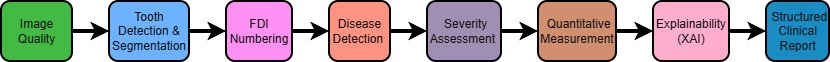
\includegraphics[width=0.95\textwidth]{fig5.jpeg}
  \caption{Task hierarchy for panoramic dental radiograph analysis, illustrating 
  the sequential stages from anatomical structure extraction to clinical report 
  generation. Early stages such as tooth segmentation and numbering achieve high 
  performance, while downstream stages including severity assessment, quantification, 
  and explainability remain underexplored, highlighting key limitations in current 
  systems.}
  \label{fig:taskhierarchy}
\end{figure*}

Early stages focus on anatomical structure identification, where systems
perform well: tooth segmentation achieves pooled sensitivity\,=\,0.92,
specificity\,=\,0.94 \cite{bonfanti2025deep}; tooth enumeration reaches
mAP50\,=\,0.978 \cite{nassiri2025yolo}. Performance drops in the middle
stages -- disease detection and severity assessment. Detection on OPG reaches only mAP50\,$\approx$\,0.61
\cite{nassiri2025yolo}, and severity staging appears in only three
of 21 C1 papers \cite{bizjak2024advancing,asadi2024detection,wang2026transformer}.
The terminal stages -- explainability and structured reporting -- were,
until 2026, the most neglected: explainability appeared in only 3 of
47 base-corpus papers (6.4\%)
\cite{chen2023deep,chen2024cariesxrays,bilal2024pdcnet}, rising to 9 of
70 (12.9\%) with the August 2026 update, and structured report
generation was absent from every system until DentFound and Balel et
al.\ \cite{zhu2026dentfound,balel2026hybrid} demonstrated it in 2026,
albeit on private data and without independent reproducibility for
DentFound. Dental AI is therefore still substantially a
sequential reasoning problem, with early-stage failures propagating into
downstream decisions. For systems targeting junior clinicians, the
absence of visual explanations removes any educational value.

\subsection{System-Level Limitations}

Five system-level limitations persist across the reviewed literature,
reflecting field-wide methodological choices:

\begin{itemize}
    \item \textbf{Task Fragmentation:} No panoramic OPG system in the
          base corpus simultaneously addresses caries detection,
          severity staging, periodontal quantification, and
          explainability. Chen et al.\ \cite{chen2023deep} achieves
          dual-disease detection with explainability -- closest to
          unified among the base corpus -- but only on periapical
          radiographs. DentFound \cite{zhu2026dentfound}, identified in
          the August 2026 update, narrows this gap further on
          panoramic radiographs by combining detection, periodontal
          findings, and post-hoc explainability in one system, but
          still without severity staging, bone-loss quantification, or
          public model weights and training data.

    \item \textbf{Severity Staging Deficit:} Asadi
          \cite{asadi2024detection}, Bizjak and Robic
          \cite{bizjak2024advancing}, and, from the 2026 update, Wang
          and Li \cite{wang2026transformer} provide caries severity
          differentiation among 21 C1 papers. For periodontal disease,
          the 2018 AAP/EFP Stages I--IV \cite{chmielewski20252018} are
          not addressed by any system using that exact taxonomy,
          though Le et al.\ and Li et al.\
          \cite{le2026automated,li2025novel} now perform related
          periodontal staging outside strict AAP/EFP terms.

    \item \textbf{Explainability Absence:} 9 of 70 papers now
          implement explainability (12.9\%, up from 6.4\% in the
          pre-2026 corpus), still contradicting field
          consensus
          \cite{nassiri2025yolo,gamal2025automated,sastika2025ai,
          ferrara2025applications,khubrani2025detection}. The EU AI Act
          and FDA guidance require transparency for high-risk systems --
          requirements 61 of 70 systems still cannot satisfy.

    \item \textbf{Dataset Fragmentation:} Approximately 60\% of the
          original base-corpus studies use private, single-center
          datasets causing heterogeneity values $I^2$\,=\,88--96\%
          \cite{iacob2025automated,albano2024artificial,bonfanti2025deep}.
          The 2026 update's largest systems remain predominantly
          private as well, though public resources such as MMOral
          \cite{hao2025mmoral} are beginning to emerge.
          Mure\c{s}anu et al.\ \cite{muresanu2024automating} documented
          22\% F1 degradation from internal to external data. No
          large-scale, multi-disease, multi-center, publicly available
          panoramic dataset with standardized annotations exists.

    \item \textbf{Clinical Workflow Disconnection:} Except for
          Schwendicke et al.\ \cite{schwendicke2021cost}
          (cost-effectiveness analysis) and Lee et al.\
          \cite{lee2025evaluation} (65-dentist usability study), no
          system evaluates AI within actual clinical workflows. Most
          produce bounding boxes without structured reports or treatment
          recommendations.
\end{itemize}
%---------------------------

\section{Background}
\label{sec:background}

\subsection{Panoramic Radiography in Clinical Dentistry}

Orthopantomography (OPG) produces a two-dimensional tomographic
representation of the curved dental arches on a flat image plane. Where
periapical or bitewing radiographs cover only limited regions, a single
panoramic image captures all 32 permanent teeth, maxilla and mandible,
and surrounding structures, making it the most information-dense
single radiographic acquisition in routine dental practice. For caries
detection, panoramic radiographs are less sensitive than bitewing for
early proximal lesions \cite{perez2024ai,bizjak2024advancing,pornprasertsuk2025clinical}.
For periodontal bone loss assessment, OPG is the standard screening
tool, enabling visualization of the alveolar crest relative to the
cemento-enamel junction (CEJ) across all teeth
\cite{jundaeng2025advanced,iacob2025automated,khubrani2025detection}.
This modality distinction directly shapes the architectural requirements
for AI systems addressing each task.

\subsection{Deep Learning Architectures}

The architectures reviewed fall into four functional families. First,
CNNs with transfer learning -- ResNet~\cite{khuwaja2024ai},
DenseNet~\cite{kaushik2025densenet201,kaushik2025densenet201,ozdemir2026enhanced},
VGG~\cite{mathur2025comparative}, EfficientNet~\cite{chen2023deep},
Inception~\cite{gamal2025automated,zancan2025ai} -- are used primarily
for classification, leveraging ImageNet pre-training to compensate for
limited dental dataset sizes. Second, YOLO-family one-stage object
detectors (YOLOv5--YOLOv9)
\cite{ayhan2025detection,nassiri2025yolo,bizjak2024advancing,muresanu2024automating,pornprasertsuk2025clinical}
dominate detection tasks for their real-time speed and strong bounding
box localization. Third, U-Net and nested variants
\cite{alharbi2023detection,asci2024deep,lim2024dual,kong2024integrating,zanini2024systematic}
are the standard for pixel-level segmentation, using skip connections to
preserve spatial detail. Fourth, transformer architectures -- ViT
\cite{bhoopalan2026self}, Swin Transformer
\cite{vannistelrooij2024combining,zhang2025reliable}, RT-DETR
\cite{karamuftuo2025panoramic} -- represent the most recent frontier,
offering global attention at higher computational cost.

\subsection{Evaluation Metrics}

A persistent challenge is metric inconsistency, which prevents direct
cross-study comparison
\cite{iacob2025automated,bonfanti2025deep,khubrani2025detection,zanini2024systematic}.
Object detection studies report mAP at IoU thresholds of 0.50 and
0.50:0.95. Segmentation studies use IoU and Dice coefficient.
Classification studies report accuracy, AUC, sensitivity, specificity,
and F1. Some studies \cite{chen2023deep,bilal2024pdcnet,zancan2025ai}
also report PPV and NPV, which have direct clinical relevance that
aggregate accuracy scores can obscure. The absence of a standardized
dental AI evaluation protocol is one of the most frequently cited
methodological gaps across the reviewed corpus
\cite{iacob2025automated,luke2025accuracy,khubrani2025detection}.

% -----------------------------------------------------------------------
\section{Caries Detection and Severity Classification (C1)}
\label{sec:caries}

Caries detection is the most extensively studied task in dental AI,
accounting for 21 of the 70 reviewed papers. The studies span object
detection, segmentation, classification, and systematic review
methodologies across panoramic, bitewing, periapical, and intraoral RGB
modalities.

\subsection{YOLO-Based Detection on Panoramic Radiographs}

Ayhan et al.~\cite{ayhan2025detection} proposed a two-stage pipeline
targeting caries beneath fixed dental prostheses (FDPs), a scenario
where metal artifacts from crowns and bridges actively obscure lesion
visibility. YOLOv7 detected FDP regions
(mAP\,=\,0.968, F1\,=\,0.956) in Stage~1; a CBAM-enhanced YOLOv7
applied to cropped ROIs then achieved caries detection with mAP\,=\,0.846
and F1\,=\,0.830 in Stage~2. The CBAM attention module produced
measurable gains on low-contrast lesion boundaries beneath metallic
artifacts.

Bizjak and Robic~\cite{bizjak2024advancing} applied a two-step YOLOv8
pipeline on the public DENTEX dataset, achieving tooth enumeration
mAP@0.5\,=\,0.95 and lesion sensitivity\,=\,0.70 (internal), 0.67
(external). That external evaluation is among the few genuine
cross-site validations in the corpus and confirms the performance drop
that single-center training typically produces. Asadi~\cite{asadi2024detection} applied Faster
R-CNN to the UFBA-UESC public dataset, achieving 94\% overall accuracy
but with a notable clinical weakness: recall for mild
caries was 0.64 versus 0.69 for severe caries -- the inverse of clinical
need, where early lesions matter most.
Pornprasertsuk-Damrongsri et al.~\cite{pornprasertsuk2025clinical}
combined YOLOv5s for tooth detection with Attention U-Net for caries
segmentation on 500 panoramic radiographs with bitewing-confirmed ground
truth, achieving Recall\,=\,0.96, F1\,=\,0.85 with Bland-Altman
agreement analysis. An example of multi-tooth carious lesion detection with severity differentiation in panoramic radiographs is shown in Fig.~\ref{fig:dentex}.

\begin{figure*}[t]
    \centering
    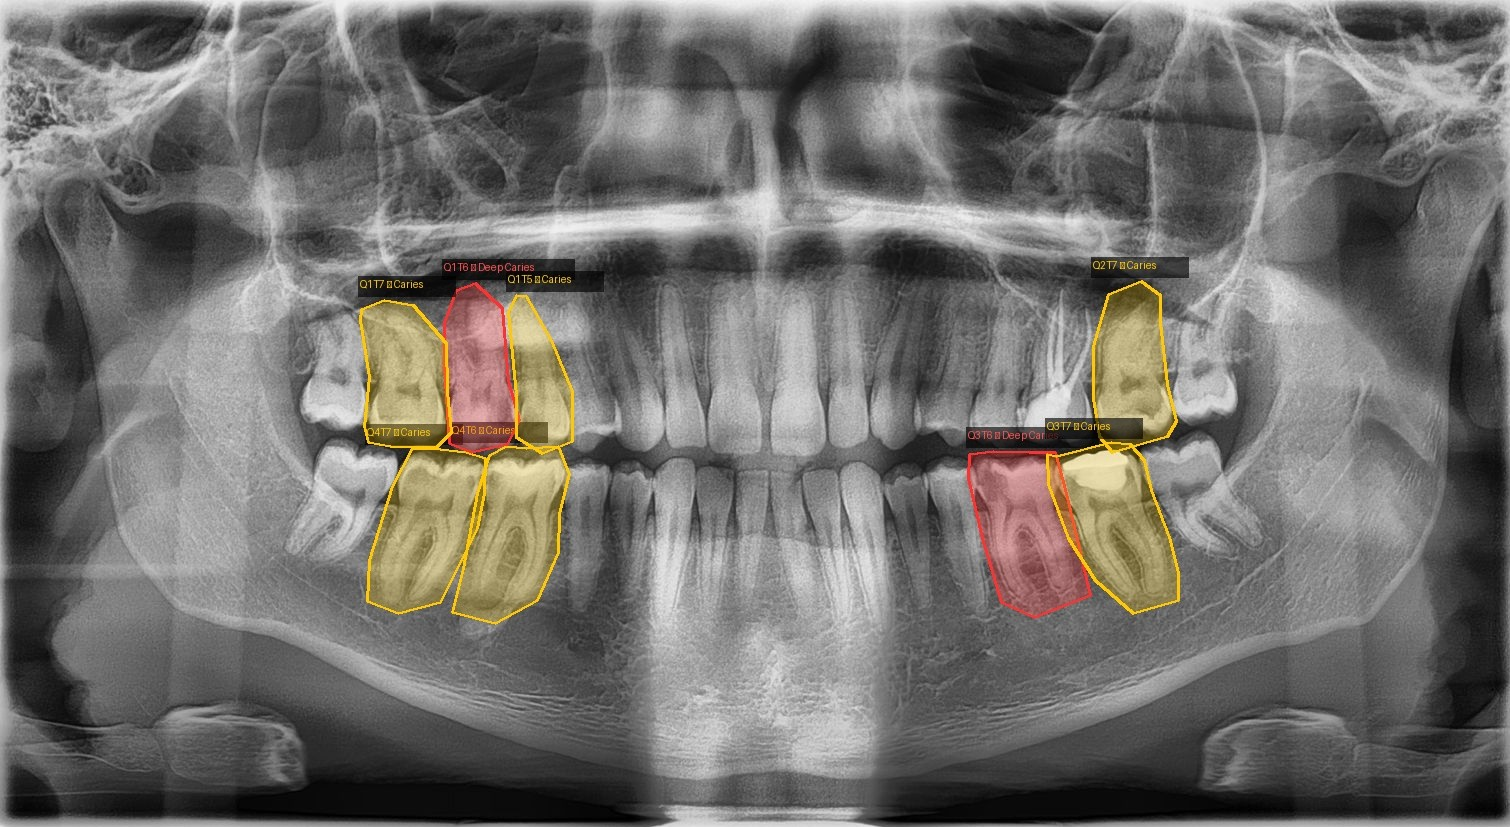
\includegraphics[width=0.65\textwidth]{fig2.jpg}
    \caption{Example panoramic radiograph with annotated carious lesions, 
    illustrating multi-instance detection and severity differentiation 
    (caries vs.\ deep caries) across multiple teeth.}
    \label{fig:dentex}
\end{figure*}

\subsection{U-Net Segmentation Approaches}

Alharbi et al.~\cite{alharbi2023detection} compared U-Net, U-Net++, and
U-Net3+ on 1,500 panoramic images. U-Net3+ achieved the best test
performance (IoU\,=\,0.67, Dice\,=\,0.60, Accuracy\,=\,0.95); its
full-scale skip connections gave a measurable advantage over standard
U-Net (Dice\,=\,0.58). The gap between training IoU (0.77) and test IoU
(0.67) reflects overfitting driven by class imbalance -- only 510 of
1,500 images contained visible cavities.

Lim et al.~\cite{lim2024dual} proposed Faster R-CNN + U-Net
(EfficientNet-B0 encoder) on 597 panoramic radiographs, achieving
IoU\,=\,0.608, Dice\,=\,0.743, Recall\,=\,0.731 on 33,752 augmented
cropped tooth images, with no severity grading or explainability.
Asci et al.~\cite{asci2024deep} applied U-Net to 6,075 pediatric
panoramic radiographs across primary, mixed, and permanent
dentition, achieving F1\,=\,0.8675, Sensitivity\,=\,0.8269,
Precision\,=\,0.9123. The results show U-Net's adaptability across
diverse tooth morphologies, though AUC\,=\,0.76 falls below the 90\%
clinical threshold. Vickram and Mathan Muthu~\cite{vickram2025extraction}
applied UNet variants to 500 dental X-ray images, achieving
Accuracy\,=\,98.03\% and Dice\,=\,96.77\%, though on a small dataset
with no external validation.


\subsection{CNN Classification and Transfer Learning}

Zancan et al.~\cite{zancan2025ai} applied InceptionResNet-v2 to 7,304
tooth-level images from 935 panoramic radiographs, achieving
accuracy\,=\,0.94 and F1\,=\,0.94 with five-fold cross-validation --
among the more rigorous validation schemes in C1. Kaushik and
Sharma~\cite{kaushik2025densenet201} applied DenseNet201 to 29,815
dental X-ray images, reporting 91\% overall accuracy alongside a
cavity-specific F1 of only 0.27, which illustrates how class imbalance
can render aggregate accuracy misleading. Ozdemir et al.~\cite{ozdemir2026enhanced}
applied DenseNet-121 to 14,498 cropped tooth images (2,303 caries /
12,195 non-caries), achieving accuracy\,=\,93.17\% and F1\,=\,87.49\%,
though without localization on full panoramic images. Khuwaja et
al.~\cite{khuwaja2024ai} evaluated YOLOv8, ResNet-50, EfficientDet, and
MobileNetV2 on 7,447 intraoral RGB smartphone images targeting mobile
diagnostics in resource-limited settings, with ResNet-50 achieving
mAP@0.50\,=\,0.670.

\subsection{Systematic Reviews and Meta-Analyses}

Albano et al.~\cite{albano2024artificial} reviewed 20 studies via
PRISMA/QUADAS-2, finding accuracy 73\%--98\% and AUC 0.84--0.98 across
CNN-based models. High heterogeneity was a consistent finding, and the
authors called for standardized datasets and multicenter validation. Luke and
Rezallah~\cite{luke2025accuracy} conducted a meta-analysis of 21 studies
(17,190 total samples); the best individual study achieved
98.8\% accuracy, but $I^2$ values of 88--96\% signal heterogeneity
severe enough to undermine pooled estimates. Zanini et
al.~\cite{zanini2024systematic} reviewed 42 studies and confirmed that
single-task formulations and absent caries severity differentiation are
field-wide patterns, not isolated oversights. Sastika and Marappan~\cite{sastika2025ai}
reviewed accuracy ranges of 85--99\% across multiple architectures and
explicitly identified Grad-CAM as a requirement in the studies surveyed.

Chen et al.~\cite{chen2024cariesxrays} introduced the CariesXrays
dataset (6,000 hospital-grade panoramic X-rays, 13,783 expert-verified
bounding boxes) alongside the FPCL architecture, achieving
AP\,=\,48.2\%, AP50\,=\,84.1\%, outperforming YOLOv8
(AP50\,=\,80.7\%). CariesXrays is the most substantial public benchmark
contribution in the C1 category.

\subsection{Bitewing Caries and Cost-Effectiveness}

Perez de Frutos et al.~\cite{perez2024ai} evaluated RetinaNet,
YOLOv5-M, and EfficientDet on 13,887 bitewing X-rays from the HUNT4
Oral Health Study, annotated by six dentists with a 197-image consensus
test set. YOLOv5-M achieved mAP\,=\,0.647, F1\,=\,0.548, matching or
surpassing individual expert annotators -- evidence that deep learning
can reach human expert performance on proximal caries detection.
Schwendicke et al.~\cite{schwendicke2021cost} combined U-Net
performance evaluation (accuracy\,=\,0.80, sensitivity\,=\,0.75 vs.\
dentist sensitivity\,=\,0.36) with a Markov lifetime cost-effectiveness
simulation on 3,686 bitewing radiographs. The analysis projected
increased tooth retention (64 vs.\ 62 years) and reduced cost per tooth
(\euro298 vs.\ \euro322), yielding ICER\,=\,$-$13.9~\euro/year,
which places AI caries detection in the cost-dominant category.

\begin{table*}[t]
\caption{Summary of Reviewed Studies --- Caries Detection and Severity Classification (C1)}
\label{tab:c1}
\centering
\small
\begin{tabular}{p{0.6cm} p{4.8cm} p{3.0cm} p{3.5cm} p{1.0cm} p{3.2cm}}
\toprule
\textbf{Ref} & \textbf{Model} & \textbf{Dataset Size} & \textbf{Best Metric} & \textbf{XAI} & \textbf{Key Gap} \\
\midrule
\cite{ayhan2025detection}   & YOLOv7 + CBAM & 1,004 OPG & mAP=0.846, F1=0.830 & None & Single-center, no XAI \\
\cite{khuwaja2024ai}        & YOLOv8, ResNet-50, EfficientDet, MobileNetV2 & 7,447 RGB & mAP@0.50=0.670 & None & RGB only, no radiographs \\
\cite{alharbi2023detection} & U-Net, U-Net++, U-Net3+ & 1,500 OPG & IoU=0.67, Dice=0.60 & None & Class imbalance, no severity \\
\cite{asci2024deep}         & U-Net & 6,075 OPG (pediatric) & F1=0.8675, AUC=0.76 & None & Below 90\% clinical threshold \\
\cite{albano2024artificial} & Systematic Review (CNNs) & 20 studies & Acc up to 0.98, AUC 0.98 & None & High heterogeneity \\
\cite{kaushik2025densenet201} & DenseNet201 & 29,815 X-rays & Acc=91\%, Cavity F1=0.27 & None & Severe class imbalance \\
\cite{chen2024cariesxrays}  & FPCL (Faster R-CNN + D2D-FPN + Contrastive) & 6,000 OPG & AP=48.2\%, AP50=84.1\% & Attn maps & No severity/periodontal \\
\cite{perez2024ai}          & YOLOv5-M, RetinaNet, EfficientDet & 13,887 bitewing & mAP=0.647, F1=0.548 & None & Bitewing only, no periodontal \\
\cite{sastika2025ai}        & Review: U-Net, ResNet, YOLOv7/v8, ensemble & Multiple studies & Acc 85--99\%, F1 87--94\% & Discussed & No original experiment \\
\cite{schwendicke2021cost}  & U-Net & 3,686 bitewing & Acc=0.80, ICER=$-$\euro13.9/yr & None & Single-center, German context \\
\cite{luke2025accuracy}     & Meta-analysis (CNNs) & 21 studies, 17,190 images & Best Acc=98.8\% & None & $I^2$=88--96\% heterogeneity \\
\cite{vickram2025extraction}& UNet, UNet+, UNet++ & 500 images & Acc=98.03\%, Dice=96.77\% & None & Small dataset, no clinical val. \\
\cite{wang2026transformer}  & Hierarchical Transformer + FPN & 3,856 OPG, 12,847 lesions & mAP=87.3\%, D1--D4 staged & Partial & Private, metallic-artifact errors \\
\cite{ghimire2025cnns}      & 12-architecture benchmark (CNN/ViT/Mamba) & DC1000 (597 OPG) & Best Dice=0.7345 (CNN) & None & Small data regime only \\
\cite{kim2026automated}     & Faster R-CNN + U-Net & 3,000 OPG (AI-Hub) & Dice=0.9482 (unverified) & None & Protocol not confirmable (paywalled) \\
\cite{zancan2025ai}         & InceptionResNet-v2 & 935 OPG / 7,304 teeth & Acc=0.94, F1=0.94 & None & No localization, no periodontal \\
\cite{lim2024dual}          & Faster R-CNN + U-Net (EfficientNet-B0) & 597 OPG & IoU=0.608, Dice=0.743 & None & No severity, no periodontal \\
\cite{zanini2024systematic} & Systematic Review (U-Net, Mask R-CNN, ResNet) & 42 studies & Various (review) & None & No severity differentiation \\
\cite{bizjak2024advancing}  & YOLOv8 two-step pipeline & 1,005 OPG + 85 external & mAP@0.5=0.95, Sens=0.70 & None & Caries only, no severity \\
\cite{asadi2024detection}   & Faster R-CNN & 1,000 OPG & Acc=94\%, Mild recall=0.64 & None & Weak mild caries detection \\
\cite{pornprasertsuk2025clinical} & YOLOv5s + Attention U-Net & 500 OPG, 14,997 teeth & Recall=0.96, F1=0.85 & None & Single-disease, no periodontal \\
\cite{ozdemir2026enhanced}  & DenseNet-121 & 14,498 tooth images & Acc=93.17\%, F1=87.49\% & None & No localization, no severity \\
\bottomrule
\end{tabular}
\end{table*}

\subsection{2026 Update: Transformer, Segmentation-Benchmark, and Staging Approaches}

An August 2026 literature update identified three further C1 studies not
available at the time of the original search. Wang and
Li~\cite{wang2026transformer} trained a 12-layer hierarchical
transformer with a multi-scale feature pyramid on a private
three-hospital corpus of 3,856 panoramic radiographs (12,847 lesions),
achieving mAP\,=\,87.3\% across caries stages with an explicit D1--D4
severity grade, per-grade sensitivity (81.3\% for the hardest D1
lesions), specificity\,=\,91.7\%, and expert-agreement
$\kappa$\,=\,0.84 on a genuine patient-level 70/15/15 held-out test
split -- one of the few C1 studies in this survey with a true
patient-level held-out test set, and a methodological bar most other
reviewed caries-severity work, including single-split validation
schemes elsewhere in this corpus, does not meet. Ghimire et
al.~\cite{ghimire2025cnns} benchmarked twelve CNN, vision-transformer,
and Mamba (state-space) architectures for caries segmentation on the
DC1000 dataset under a controlled 497/100 train/test protocol,
finding a plain CNN (DoubleU-Net, Dice\,=\,0.7345) outperformed every
transformer and Mamba variant tested -- a useful ceiling estimate for
contextualizing unusually high caries-segmentation Dice scores
elsewhere in the literature. Kim et al.~\cite{kim2026automated}
reported a two-stage Faster R-CNN + U-Net caries segmentation pipeline
on 3,000 panoramic radiographs from the Korean AI-Hub corpus with
Dice\,=\,0.9482; this figure is markedly higher than every other
caries-segmentation result in this survey, and because the evaluation
protocol is behind a publisher paywall it could not be independently
confirmed, so it is reported here with that explicit caveat rather than
as a verified state of the art.

% -----------------------------------------------------------------------
\section{Periodontal Disease and Alveolar Bone Loss Detection (C2)}
\label{sec:perio}

Periodontal disease detection from radiographs requires quantifying the
spatial relationship between anatomical landmarks -- specifically the
distance between the cemento-enamel junction (CEJ) and the alveolar
bone crest -- across all teeth in the panoramic image. This task demands
precise spatial localization and continuous measurement rather than
binary classification. Eighteen papers in the C2 category reflect a
less mature but rapidly advancing subfield.

\subsection{Clinical Foundation}

Chmielewski et al.~\cite{chmielewski20252018} provide essential clinical
context: the 2018 AAP/EFP classification defines periodontitis
stages~I--IV and grades~A--C based on bone loss percentage, probing
depth, tooth loss, and risk factors. Across 11 clinical studies covering
459 cases and 852 examiners, staging accuracy peaked at 90\% but
inter-examiner agreement remained variable. This is precisely the
subjectivity problem that AI systems could address -- provided they
produce quantitative, staged outputs aligned with the 2018 criteria,
rather than a binary bone loss label. Fig.~\ref{fig:perio} illustrates
the spatial nature of periodontal bone loss assessment, which requires
accurate identification of landmarks such as the CEJ and alveolar bone
crest.

\begin{figure*}[t]
    \centering
    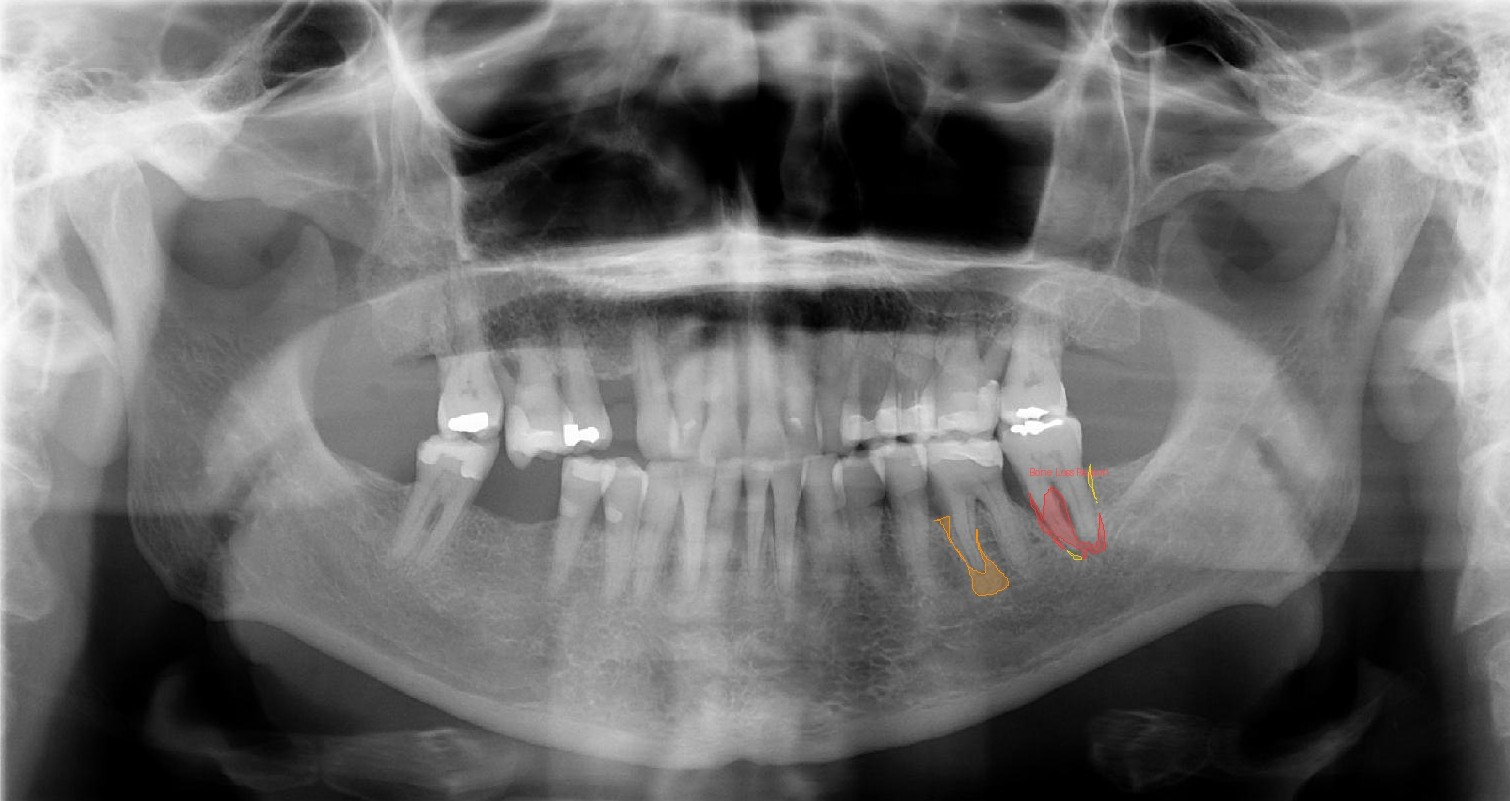
\includegraphics[width=0.65\textwidth]{fig3.jpg}
    \caption{Example panoramic radiograph illustrating periodontal bone 
    loss regions. Accurate assessment requires spatial measurement between 
    the cemento-enamel junction and alveolar bone crest.}
    \label{fig:perio}
\end{figure*}

\subsection{Landmark Detection and Bone Loss Quantification}

Jundaeng et al.~\cite{jundaeng2025advanced} reported the most
technically complete periodontal AI system in the reviewed corpus. Their
dual YOLOv8 pipeline on 2,000 panoramic radiographs achieved tooth
segmentation (Accuracy\,=\,0.97, mAP50\,=\,0.92) and CEJ/bone level
detection (Accuracy\,=\,0.98, Sensitivity\,=\,1.0, Specificity\,=\,0.98,
F1\,=\,0.90, mAP50\,=\,0.995). A sensitivity of 1.0 for bone level
detection carries practical weight: missed bone loss in a screening
context is more harmful than a false positive. Limitations include
single-center data, images of uniformly high quality, and no caries
integration or explainability.

Iacob et al.~\cite{iacob2025automated} synthesized evidence from 20
diagnostic accuracy studies covering 141,166 radiographs through
PRISMA/QUADAS-2. U-Net, YOLO, ResNet, ConvNeXt, and DeNTNet have each
been applied, but heterogeneity across studies prevents reliable
pooling. Khubrani et al.~\cite{khubrani2025detection} meta-analyzed 30
studies using APPRAISE-AI, reporting pooled sensitivity\,=\,87\%,
specificity\,=\,76\%, accuracy\,=\,84\% -- figures that are useful as
baselines but insufficient for autonomous clinical use.

Mathur et al.~\cite{mathur2025comparative} applied VGG-16 to 1,874
panoramic radiographs for binary bone loss classification
(accuracy\,=\,89.27\%, sensitivity\,=\,83.27\%). This approach, the
most common in C2, is also the most clinically limited: it produces no
staging information. Cerda Mardini et al.~\cite{cerda2024determining}
attempted quantitative staging on 500 panoramic radiographs, reporting
F1\,=\,0.29 for light-to-moderate bone loss and F1\,=\,0 for severe bone
loss. The results honestly document how difficult quantitative staging
is, and the model's failure on the most clinically critical severity
class is worth noting. Kong et al.~\cite{kong2024integrating} integrated
SRGAN super-resolution preprocessing with U-Net for bone loss
segmentation (Dice\,=\,0.91, IoU\,=\,84.9\%), the strongest segmentation
metrics in C2. The results suggest that preprocessing quality directly
affects segmentation accuracy, though the 698-image dataset is small and
no disease staging is included.

Wimalasiri et al.~\cite{wimalasiri2025ai} applied YOLOv8x and Keypoint
R-CNN to 1,000 intraoral periapical X-rays, achieving ICC\,=\,0.80 for
severity and 87\% for bone loss pattern classification (horizontal
vs.\ vertical). Pattern classification is absent from all other reviewed
systems and has direct prognostic value for surgical planning. Tian et
al.~\cite{tian2025development} developed the PAN-POL mathematical model
validated on 290 panoramic patients, achieving ICC\,=\,0.83, though
this is a rule-based rather than a deep learning approach.

\subsection{Periodontitis Classification}

Bilal et al.~\cite{bilal2024pdcnet} proposed PDCNET -- a custom
five-block CNN with Grad-CAM explainability -- and evaluated it against
EfficientNet-B0, DenseNet-201, VGG-16, VGG-19, Inception-V3, and
MobileNet on a Kaggle dataset augmented with SMOTE-Tomek, achieving
accuracy\,=\,98.39\%, AUC\,=\,99.79\%, F1\,=\,98.31\%. These are the
highest classification metrics in C2, though the original sample of
50 positive and 50 negative cases raises serious concerns about
statistical reliability. The paper is useful for demonstrating the
feasibility of Grad-CAM in periodontal AI.
Ferrara et al.~\cite{ferrara2025applications} reviewed 13 periodontal
deep learning studies via PRISMA/QUADAS-2, reporting accuracy ranges of
73\%--98.6\% and noting that explainable AI is absent from every system
reviewed. Lee et al.~\cite{lee2025evaluation} assessed AI alveolar bone
loss measurement usability through a survey of 65 dentists on 550
bitewing images -- one of the few clinical usability studies in the
entire corpus.

Kim et al.~\cite{kim2024unsupervised} proposed an unsupervised few-shot
learning architecture combining UNet, CVAE, and clustering methods
(k-means/DBSCAN/GMM) on 1,372 panoramic radiographs. The approach
achieved a 14\% improvement over supervised ViT, suggesting that
label-efficient learning may be a practical path forward in
data-scarce dental AI settings.
Karamuftuo\u{g}lu et al.~\cite{karamuftuo2025panoramic} benchmarked
YOLOv12x, RT-DETR-L, and RT-DETR-X on a 387-image pediatric panoramic
dataset for furcation lesion detection, achieving mAP@0.5\,=\,0.434.
The modest result reflects both the difficulty of the task and the
constraints of small single-center datasets.

\begin{table*}[t]
\caption{Summary of Reviewed Studies --- Periodontal Disease and Bone Loss (C2)}
\label{tab:c2}
\centering
\small
\begin{tabular}{p{0.6cm} p{4.5cm} p{3.0cm} p{3.8cm} p{1.0cm} p{2.8cm}}
\toprule
\textbf{Ref} & \textbf{Model} & \textbf{Dataset Size} & \textbf{Best Metric} & \textbf{XAI} & \textbf{Key Gap} \\
\midrule
\cite{jundaeng2025advanced}  & Dual YOLOv8 (teeth + CEJ/bone) & 2,000 OPG & mAP50=0.995, Sens=1.0 & None & Single-center, no caries \\
\cite{chmielewski20252018}   & Clinical review (no ML) & 459 cases, 852 examiners & Stage acc=90\% & None & No AI system proposed \\
\cite{iacob2025automated}    & Systematic Review (CNN, YOLO, U-Net) & 141,166 radiographs & Various (review) & None & High heterogeneity \\
\cite{mathur2025comparative} & VGG-16 (transfer learning) & 1,874 OPG & Acc=89.27\% & None & Binary only, no staging \\
\cite{khubrani2025detection} & Meta-analysis (CNN, YOLO, U-Net, SVM) & 30 studies & Sens=87\%, Spec=76\% & None & Pooled heterogeneity \\
\cite{tian2025development}   & PAN-POL mathematical model & 290 PAN patients & ICC=0.83 & None & Not deep learning, manual \\
\cite{lee2025evaluation}     & Faster R-CNN + DeepLab v3+ & 550 bitewing & Acc=82--87\% (severe) & None & Bitewing only, no OPG \\
\cite{cerda2024determining}  & Hybrid DCNN (Xception) + rule-based PBL & 500 OPG & F1=0.29 (lt-mod), F1=0 (severe) & None & Fails on severe PBL \\
\cite{wimalasiri2025ai}      & YOLOv8x + Keypoint R-CNN & 1,000 IOPA & ICC=0.80, Pattern Acc=87\% & None & Periapical only, no OPG \\
\cite{kong2024integrating}   & SRGAN + U-Net & 698 OPG & Dice=0.91, IoU=84.9\% & None & No severity, small dataset \\
\cite{ferrara2025applications}& Systematic Review (CNNs, hybrid) & 13 studies & Acc 73--98.6\% & None & No XAI in any reviewed study \\
\cite{bilal2024pdcnet}       & PDCNET (custom CNN) + Grad-CAM & 50+50 orig (SMOTE aug.) & Acc=98.39\%, AUC=99.79\% & Grad-CAM & Dataset too small \\
\cite{karamuftuo2025panoramic} & YOLOv12x, RT-DETR-L, RT-DETR-X & 387 OPG (pediatric) & mAP@0.5=0.434 & None & Small dataset, modest mAP \\
\cite{kim2024unsupervised}   & UNet + CVAE + k-means/DBSCAN/GMM & 1,372 OPG & +14\% over supervised ViT & None & No bounding boxes \\
\bottomrule
\end{tabular}
\end{table*}

\subsection{2026 Update: Keypoint Staging and Multicenter Validation}

Four further C2 studies were identified in the August 2026 update, and
they represent the strongest periodontal evidence in the entire corpus.
Le et al.~\cite{le2026automated} proposed a YOLOv11 six-keypoint
pipeline for automated periodontitis diagnosis and staging on 607
panoramic radiographs, reporting segmentation
precision\,=\,0.981/recall\,=\,0.984/F1\,=\,0.983/mAP50\,=\,0.994,
keypoint mAP50\,$>$\,0.958, and per-tooth-type PCC/ICC agreement for
radiographic bone loss -- directly answering the quantification gap
this survey identifies in Section~\ref{sec:taxonomy}. Li et
al.~\cite{li2025novel} introduced HC-Net+, evaluated on a multicenter
cohort with AUROC\,=\,94.2\% against a specialist AUROC of 85.6\% and
AUROC\,=\,0.967 on a second external validation cohort, with CAM-based
explainability and specialist agreement $\kappa$\,=\,0.64; the authors
also report that 20.6\% of Stage~II cases were missed even by this
system, a clinically important caveat that should temper the headline
AUROC. G\"uner et al.~\cite{guner2026fractal} synthesized 80 studies on
fractal analysis and AI for radiographic bone loss detection under a
QUADAS-2/PROSPERO-registered protocol (PROSPERO 1278324), providing the
most current systematic evidence base for this subfield. Lee et
al.~\cite{lee2025radiographic} meta-analyzed 23 further studies
comparing binary versus staged periodontitis classification across
imaging modalities, reporting pooled sensitivity, specificity, and AUC
separately by modality and by binary-versus-staging task -- direct
supporting evidence for this survey's repeated observation that binary
detection and true clinical staging are different problems with
different, generally lower, performance ceilings for the latter.
Together,
these three works are the first in this survey's corpus to combine
periodontal severity staging with any form of external or multicenter
validation, directly narrowing -- though not closing -- Gap~2 and
Gap~4 as defined in Section~\ref{sec:gaps}.

% -----------------------------------------------------------------------
\section{Multi-Task and End-to-End OPG Diagnosis (C3)}
\label{sec:multitask}

Fourteen papers address multiple diagnostic tasks within a single
pipeline applied to panoramic radiographs -- the architectural
direction most consistent with real clinical utility.

Chen et al.~\cite{chen2023deep} report the most clinically complete
dual-disease system in the corpus, combining YOLOv7 for tooth
localization with EfficientNet-B0 for simultaneous multi-label
classification of periodontitis and dental caries on periapical X-rays,
with Grad-CAM visualization. EfficientNet-B0 achieved ROC AUC\,=\,98.67\% for
periodontitis and 98.31\% for dental caries with 10-fold
cross-validation. The critical limitation is modality: periapical, not
panoramic.

Nassiri and Akhloufi~\cite{nassiri2025yolo} compared YOLO
v5--v9 on DENTEX across quadrant segmentation, tooth enumeration, and
disease detection. YOLOv9e-seg achieved mAP50\,=\,0.978 for tooth
enumeration and 0.959 for segmentation, while pathology detection peaked
at mAP50\,=\,0.61 -- confirming that structural tasks are tractable
while pathology detection remains the harder problem.

Van Nistelrooij et al.~\cite{vannistelrooij2024combining} combined
OdontoAI and DENTEX datasets with Mask DINO (ViT backbone) and Swin-B
Transformer, achieving FROC\,=\,0.988 for tooth segmentation and
AUC\,=\,0.996 for impacted teeth, the strongest tooth-level assessment
results reviewed. A 40-second inference time per image is the primary
barrier to clinical use. Gamal et
al.~\cite{gamal2025automated} demonstrated that a weighted average
ensemble of CNN architectures (Custom CNN, ResNet-50, InceptionV3,
DenseNet121, VGG19) achieves accuracy\,=\,92.93\% on 1,814 cropped
tooth images. ESRGAN super-resolution preprocessing contributed roughly
3\% of that accuracy gain.

Mure\c{s}anu et al.~\cite{muresanu2024automating} provided the most
methodologically transparent external validation in C3: YOLOv8 tested
on a Romanian clinical dataset showed internal F1\,=\,0.60 degrading to
external F1\,=\,0.47 -- a 22\% drop that directly measures the
generalization cost of single-center training.
Bhoopalan et al.~\cite{bhoopalan2026self} applied ViT and
Swin Transformer to 5,098 OPG images, achieving ViT accuracy\,=\,96\%,
precision\,=\,95.8\%, recall\,=\,96.2\%. These are strong results for
image-level classification, though the system provides neither
localization nor segmentation. Zhou et al.~\cite{zhou2025deep} reviewed
datasets, methodologies, and emerging challenges in dental
image analysis, reinforcing the need for standardization across the
field.

\subsection{2026 Update: Vision-Language Systems and Benchmarks}

The August 2026 update identified seven further C3 systems, and they
change the framing of this survey's central claim. Zhu et
al.~\cite{zhu2026dentfound} introduced DentFound, an instance-guided
vision-language model that injects tooth-instance masks as visual
embeddings into a transformer-based VLM to produce tooth-level
diagnosis and free-text radiology reports across 98 disease categories
and 11 post-treatment categories. DentFound was trained and validated
on a private multi-hospital corpus exceeding 101,000 patients across
four clinical centers, with an expert reader study on 595 panoramic
radiographs in which 12 dentists and radiologists rated
DentFound-generated reports as superior to or comparable with
human-written reports, and with broader diagnostic coverage. It
provides post-hoc Grad-CAM-style regional-response explainability tied
to individual generated findings and identifies tooth position across
52 sites using FDI-style numbering. This is, to our knowledge, the
most clinically integrated dental panoramic system published to date.
It is also, on close reading, not the system this survey's original
central claim needs to rule out: the accessible portions of the paper
report no quantitative caries severity staging (no D1--D4 or
equivalent grade) and no numeric periodontal bone-loss quantification
(no CEJ-to-crest distance, percentage bone loss, or AAP/EFP stage);
its outputs are narrative findings rather than the graded,
measurement-level outputs this survey's taxonomy requires in
Section~\ref{sec:taxonomy}. Reproducibility is also asymmetric: the
inference code is released under an Apache~2.0 license, but neither
fine-tuned model weights nor the training data are public, so the
system cannot currently be independently re-run or externally
audited by a third party. An Author Correction was published on 8~July
2026; readers relying on specific DentFound figures should consult it.

Three concurrent benchmark efforts test whether general-purpose
vision-language models can substitute for task-specific pipelines like
DentFound's or the one proposed in this survey, and all three answer
no. Hao et al.~\cite{hao2025mmoral} released MMOral, an instruction and
benchmark dataset of 20,563 annotated panoramic radiographs (1.3
million instruction-following instances), and evaluated 64 large
vision-language models zero-shot: the best proprietary model, GPT-4o,
reached only 43.3\% accuracy, and a medical-specific model
(HealthGPT-XL32) reached only 39.7\%; supervised fine-tuning on MMOral
lifted a mid-sized open model from 21.5\% to 46.2\%. Li et
al.~\cite{li2026pandent} introduced PanDent, 9,524 expert-validated
orthopantomograms for tooth-level structure-language consistency,
reporting that current MLLMs produce fluent but clinically
inconsistent reports with substantial fine-grained localization
errors. Jha et al.~\cite{jha2026dentiask} introduced DentiAsk, a
10,000-question VQA benchmark spanning descriptive, spatial, and
numerical-quantification reasoning tiers, and found that models
degrade sharply on exactly the spatial-localization and counting
questions that panoramic diagnosis depends on. Taken together, these
benchmarks are direct evidence that deterministic, task-specific
detection-plus-classification pipelines -- of the kind formalized in
this survey's taxonomy (Section~\ref{sec:taxonomy}) -- remain
necessary: general VLMs are not yet a substitute for explicit
tooth-level geometric grounding.

Two further 2026 systems are methodologically relevant without
matching DentFound's scale. Balel et al.~\cite{balel2026hybrid}
paired YOLOv12 detection/segmentation with locally hosted LLMs
(DeepSeek~R1, Mistral, Llama~3.2) to generate structured reports from
30,954 panoramic radiographs, and found that commercial cloud LLMs
(ChatGPT, Gemini, cloud DeepSeek~R1) hallucinated findings in 100\% of
generated reports, versus 30 hallucinations across 50 reports for the
best local, structured-JSON-grounded pipeline -- a direct caution for
any future report-generation component of a system like ours.
Eftimie et al.~\cite{eftimie2025tooth} (published under the name
Sorana Muresanu on an earlier preprint) reported a two-stage
YOLOv11-then-RT-DETR pipeline that detects, segments, and assigns 14
pathology categories to individual teeth, evaluated on both an
institutional corpus and, as a cross-dataset generalization test, the
public Tufts Dental Database -- the closest published architectural
analogue to the detect-then-classify system design formalized in this
survey's taxonomy (Section~\ref{sec:taxonomy}), and one of the only C3
systems to report a working lesion-to-tooth assignment step end to
end. Alnasser et
al.~\cite{alnasser2026advanced} compared five CNN backbones on a
35-class, 10,580-image panoramic dataset with Grad-CAM explainability,
reaching 97.5\% whole-image accuracy; because the evaluation uses a
random rather than patient-level split on an aggregated public-mirror
dataset, near-duplicate leakage cannot be excluded and the figure
should be read as an upper bound rather than a clean generalization
estimate.

%----------------------------------------------------------
\section{Explainable AI in Dental Diagnostics (C4)}
\label{sec:xai}

Of the original 47-paper base corpus, only three reported any
explainability output: Chen et al.~\cite{chen2023deep} use Grad-CAM for
dual-disease classification on periapical X-rays; Bilal et
al.~\cite{bilal2024pdcnet} apply Grad-CAM to periodontal disease
classification; and Chen et al.~\cite{chen2024cariesxrays} include
attention visualization in feature maps for caries detection. That
constituted \textbf{6.4\%} of the base corpus -- a figure that directly
quantified the explainability deficit in dental AI as of March 2025.

The August 2026 update raises this to \textbf{9 of 70 papers
(12.9\%)}. Wang and Li~\cite{wang2026transformer} provide attention
visualization maps alongside their caries-staging transformer, though
the authors themselves describe formal explainability as future work
rather than a validated method. DentFound~\cite{zhu2026dentfound}
generates post-hoc regional-response visualizations tied to individual
report findings, evaluated qualitatively by clinicians rather than
against ground-truth localization. Alnasser et
al.~\cite{alnasser2026advanced} apply Grad-CAM across a 35-class
classifier, and Li et al.~\cite{li2025novel} report CAM-based
explanations alongside HC-Net+'s periodontitis staging. Two further
2026 papers are explicitly about explainability rather than merely
using it: George et al.~\cite{george2026explainable} propose a
two-stage YOLOv8-plus-ResNet-50 framework for pericoronitis assessment
with Grad-CAM shown to reach 84\% concordance with radiologist
annotations on a 50-image reader check; Ren and
Chen~\cite{ren2026dualbranch} compare five CAM-family methods for
caries classification explainability and find XGrad-CAM the strongest,
though the modality used is not confirmed to be panoramic and should
be treated cautiously in that respect. Mehta et
al.~\cite{mehta2026explainability} synthesize explainability, bias, and
generalizability across 11 dental-imaging studies, reporting accuracy
figures up to 95.1\% alongside accuracy-trustworthiness correlations
ranging from 0.367 to 0.987 depending on study design -- a useful
reminder that high accuracy and high trustworthiness are not the same
property and do not co-vary reliably across this literature. Even at
12.9\%, explainability implementation remains a minority practice, and
no method beyond the CAM family (SHAP, LIME, or transformer
attention-based interpretability) has been applied to panoramic dental
diagnosis anywhere in this corpus.

Gradient-weighted Class Activation Mapping (Grad-CAM) generates a
coarse localization map of the image regions most influential for a
CNN prediction. In dental diagnostics, it serves three practical
functions: (i)~it allows clinicians to verify that the model attends to
anatomically plausible regions; (ii)~it can function as a visual
teaching tool for junior clinicians learning radiographic interpretation;
and (iii)~it creates an audit trail relevant to the EU AI Act and FDA
guidance on AI/ML-based medical devices, both of which classify AI
diagnostic tools as high-risk systems requiring transparency and human
oversight \cite{chen2023deep}.

Field consensus holds that explainability is necessary for clinical
adoption
\cite{nassiri2025yolo,gamal2025automated,sastika2025ai,ferrara2025applications},
yet the implementation rate remains under 13\%. For systems targeting
junior clinicians and dental students, this is more than an oversight
-- a visual justification is what transforms AI-assisted diagnosis
from prediction into education. SHAP, LIME, and transformer attention
visualization remain almost entirely unused in dental AI outside a
handful of unvalidated attention-map visualizations; transformer
attention maps are already intrinsic to the architecture and add no
computational overhead \cite{bhoopalan2026self}.


%------------------------------------------------------------------

\section{Comparative Analysis of Representative Methods}
\label{sec:comparison}

\begin{table*}[t]
\renewcommand{\arraystretch}{1.4}
\caption{Comparison of Representative Deep Learning Methods for Dental
Radiograph Analysis. Performance metrics are reported as provided in
the respective studies and are not directly comparable due to variations
in tasks, datasets, and evaluation protocols.}
\label{tab:comparison}
\centering
\scriptsize
\setlength{\tabcolsep}{3pt}
\begin{tabular}{p{0.5cm} p{2.0cm} p{1.3cm} p{2.2cm} p{1.1cm} p{2.4cm} p{1.6cm} p{0.6cm} p{1.3cm} p{2.2cm}}
\toprule
\textbf{Ref} & \textbf{Task} & \textbf{Scope} &
\textbf{Dataset (Size)} & \textbf{Modality} & \textbf{Model} &
\textbf{Best Metric} & \textbf{XAI} &
\textbf{Clinical Val.} & \textbf{Key Limitation} \\
\midrule
\cite{ayhan2025detection}        & Caries Detection             & Single-task & Private OPG (1,004)             & OPG      & YOLOv7 + CBAM           & mAP=0.846        & No      & Internal & No external validation \\
\cite{jundaeng2025advanced}      & Bone Loss + Periodontal      & Multi-task  & Private OPG (2,000)             & OPG      & YOLOv8                  & mAP50=0.995      & No      & Internal & Single-center dataset \\
\cite{chen2023deep}              & Multi-disease Detection      & Multi-task  & Periapical (11k)                & X-ray    & YOLOv7 + EfficientNet   & AUC$\approx$98\% & Yes     & Internal & Not panoramic \\
\cite{alharbi2023detection}      & Caries Segmentation          & Single-task & DNS (1,500)                     & OPG      & U-Net3+                 & Dice=0.60        & No      & Internal & Small dataset \\
\cite{asci2024deep}              & Caries Segmentation          & Single-task & Pediatric OPG (6,075)           & OPG      & U-Net                   & F1=0.867         & No      & Internal & No severity staging \\
\cite{gamal2025automated}        & Multi-disease Classification & Multi-task  & Roboflow (1,075)                & OPG      & CNN Ensemble            & Acc=92.9\%       & No      & Internal & No explainability \\
\cite{chen2024cariesxrays}       & Caries Detection             & Single-task & CariesXrays (6,000)             & OPG      & Faster R-CNN            & AP50=84.1\%      & Partial & Internal & Single-disease \\
\cite{perez2024ai}               & Caries Detection             & Single-task & HUNT4 (13k)                     & Bitewing & YOLOv5                  & mAP=0.647        & No      & External & Not panoramic \\
\cite{nassiri2025yolo}           & Multi-task OPG Analysis      & Multi-task  & DENTEX ($\sim$1,000)            & OPG      & YOLOv9-seg              & mAP=0.978        & No      & Internal & Limited pathology \\
\cite{vannistelrooij2024combining}& Tooth + Diagnosis            & Multi-task  & OdontoAI (1,661) + DENTEX (682) & OPG      & Mask DINO + Swin        & FROC=0.988, AUC=0.996 & No & Internal & Slow pipeline (40s/image) \\
\cite{zancan2025ai}              & Tooth + Caries               & Multi-task  & 935 PAN / 7,304 teeth           & OPG      & InceptionResNet         & Acc=0.94, F1=0.94 & No      & Internal & No localization \\
\cite{lim2024dual}               & Caries Segmentation          & Single-task & 597 PAN                         & OPG      & Faster R-CNN + U-Net    & Dice=0.743       & No      & Internal & Single-disease \\
\cite{bizjak2024advancing}       & Caries Detection             & Single-task & DENTEX + external               & OPG      & YOLOv8                  & mAP=0.95         & No      & External & No segmentation \\
\cite{asadi2024detection}        & Caries Severity              & Single-task & 1,000 PAN                       & OPG      & Faster R-CNN            & Acc=94\%         & No      & Internal & Weak mild detection \\
\cite{pornprasertsuk2025clinical}& Caries Detection             & Multi-stage & 500 PAN                         & OPG      & YOLOv5 + U-Net          & Recall=0.96      & No      & Internal & Single-disease \\
\cite{mathur2025comparative}     & Bone Loss Classification     & Single-task & 1,874 OPG                       & OPG      & VGG-16                  & Acc=89.27\%      & No      & Internal & No localization \\
\cite{lee2025evaluation}         & Bone Loss Detection          & Single-task & Bitewing (550)                  & Bitewing & Faster R-CNN + DeepLab  & Acc$\approx$85\% & No      & Internal & Limited modality \\
\cite{wimalasiri2025ai}          & Bone Loss Severity           & Single-task & DenPAR (1,000)                  & IOPA     & YOLOv8 + KRCNN          & ICC=0.80         & No      & Internal & Not panoramic \\
\cite{kong2024integrating}       & Bone Loss Segmentation       & Single-task & CBNUH (100) + Kaggle ($\sim$600)& OPG      & SRGAN + U-Net           & Dice=0.91        & No      & Internal & No detection \\
\cite{muresanu2024automating}    & Multi-disease Detection      & Single-task & Multi-center panoramic          & OPG      & YOLOv8                  & F1=0.60→0.47     & No      & External & Poor generalization \\
\cite{zhang2025reliable}         & Tooth Segmentation           & Multi-stage & Tufts + O2PR                    & OPG      & Mask R-CNN + YOLO       & AP50=97.3\% (Tufts), 98.1\% (O2PR) & No & Internal & No disease labels \\
\cite{bonfanti2025deep}          & Tooth Segmentation Review    & Review      & 20 studies                      & Multi    & CNNs                    & Sens=0.92        & No      & Review   & High heterogeneity \\
\cite{khubrani2025detection}     & Bone Loss Review             & Review      & 30 studies                      & Multi    & CNNs                    & Acc=84\%         & No      & Review   & No standardization \\
\cite{zhou2025deep}              & Deep Learning Survey         & Review      & 260 studies                     & Multi    & Various                 & ---              & No      & Review   & No unified system \\
\cite{bilal2024pdcnet}           & Periodontal Classification   & Single-task & Kaggle ($\sim$1,000)            & X-ray    & PDCNET                  & Acc=98.39\%      & Yes     & Internal & No localization \\
\end{tabular}
\end{table*}

Table~\ref{tab:comparison} restricts comparison to the 25 studies that
report a single clear headline metric directly comparable across
tasks; the newer 2026 systems discussed in Sections~\ref{sec:multitask}
and~\ref{sec:xai} are deliberately excluded here because several of
them (DentFound in particular) report reader-study ratings and
narrative-generation quality rather than a single quantitative metric,
and forcing such results into a single ``Best Metric'' cell would
misrepresent them. Within these 25 studies, task scope splits into 14
single-task, 6 multi-task, 2 multi-stage, and 3 review/survey works --
confirming that single-disease, single-task formulations remain the
dominant experimental design even among the field's most cited
results. Validation practice is similarly concentrated: 19 of the 25
report only internal (same-center) validation, 3 report a genuine
external or cross-site cohort
(\cite{perez2024ai,bizjak2024advancing,muresanu2024automating}), and 3
are themselves reviews. Explainability is essentially absent from this
representative subset, with only 2 studies applying a validated
Grad-CAM output and 1 further study showing unvalidated feature-map
attention -- the remaining 22 provide no interpretability output at
all.

Modality is heavily skewed toward panoramic imaging (17 of 25 OPG,
with 2 bitewing, 2 periapical/X-ray, 1 intraoral periapical, and 3
multi-modality reviews), which supports treating panoramic radiographs
as the primary modality for this survey while noting that comparisons
against bitewing- or periapical-only studies elsewhere in this table
are not strictly like-for-like. Reported metrics are also
inconsistent enough to limit direct comparison: 8 of the 25 studies
report an mAP-family detection metric, 7 report accuracy or AUC, 3
report Dice, and the remaining 7 each report a distinct metric (F1,
recall, ICC, or sensitivity) used nowhere else in the table. This
metric fragmentation, more than any single result, is why
Table~\ref{tab:comparison} is presented as a qualitative landscape
rather than a ranked comparison.

Finally, the table makes the severity-and-quantification gap
concrete: of these 25 representative studies, only
Asadi~\cite{asadi2024detection} performs any caries severity
differentiation, and none reports a bone-loss quantity (a millimeter
distance, a percentage, or an AAP/EFP stage) on panoramic imaging
specifically -- Wimalasiri et al.'s ICC-based severity result
\cite{wimalasiri2025ai} is the closest analogue in this table, but it
is reported on intraoral periapical radiographs, not panoramic ones.
As Section~\ref{sec:multitask} discusses, this specific gap is
narrowed, though not fully closed on panoramic imaging, by Le et
al.'s 2026 keypoint-based bone-loss quantification work
\cite{le2026automated} and Wang and Li's 2026 caries-staging
transformer \cite{wang2026transformer}, neither of which was available
at the time the base corpus for this table was assembled.

% -----------------------------------------------------------------------
\section{Datasets, Benchmarks, and Clinical Validation (C5)}
\label{sec:datasets}

Dataset availability and quality are the most frequently cited
limitations across all 70 reviewed papers. The key public
benchmarks in the field are as follows:

\begin{itemize}
  \item \textbf{DENTEX}: 1,005 panoramic radiographs with quadrant,
        tooth, and pathology annotations from three institutions
        \cite{nassiri2025yolo,vannistelrooij2024combining,bizjak2024advancing}.
  \item \textbf{CariesXrays}: 6,000 hospital-grade panoramic images
        with 13,783 caries bounding boxes \cite{chen2024cariesxrays}.
  \item \textbf{Tufts Dental Database}: Approximately 1,000 panoramic
        radiographs with tooth segmentation masks
        \cite{cerda2024determining,kim2024unsupervised,zhang2025reliable,yaswanth2025automated},
        with a January 2026 benchmark reporting binary tooth-segmentation
        Dice\,=\,0.9259 as a current reference point
        \cite{yalim2026comparative}.
  \item \textbf{HUNT4 Oral Health Study}: 13,887 bitewing X-rays with
        six-dentist annotations and a 197-image consensus set
        \cite{perez2024ai}.
  \item \textbf{UFBA-UESC}: 4,000 panoramic images
        \cite{asadi2024detection}.
  \item \textbf{MMOral} (2025): the largest public panoramic resource
        identified in this survey -- 20,563 annotated radiographs with
        1.3 million instruction-following instances, released as a
        vision-language instruction and benchmark dataset rather than
        a conventional detection/classification set
        \cite{hao2025mmoral}.
  \item \textbf{BRAR-anchored multimodal dataset} (2025): 1,104
        patients with inter-rater agreement $\kappa$\,=\,0.88 and a
        published EfficientNet-B0 baseline (accuracy\,=\,63.3\%),
        intended as a shared benchmark for periodontal bone-loss work
        \cite{xia2025brar}.
\end{itemize}

Despite these contributions, roughly 60\% of the original 47-paper
base corpus relied on private, single-center institutional data.
Systematic reviews
\cite{iacob2025automated,albano2024artificial,luke2025accuracy,bonfanti2025deep,khubrani2025detection}
consistently report $I^2$ heterogeneity values of 88--96\%, which is the
primary barrier to reliable evidence synthesis. The performance
degradation from internal to external validation documented by
Mure\c{s}anu et al.~\cite{muresanu2024automating} -- F1 dropping from
0.60 to 0.47 -- directly measures the cost of single-center training.
The August 2026 update does not reverse this pattern: DentFound's
101,000-patient training corpus, Wang and Li's three-hospital caries
corpus, and Balel et al.'s 30,954-image reporting corpus
\cite{zhu2026dentfound,wang2026transformer,balel2026hybrid} are all
private institutional data, even as MMOral and the BRAR dataset show
that large \emph{public} resources are now starting to appear.

Two 2026 systematic reviews assess how close the field actually is to
clinical deployment rather than benchmark performance alone. Wang et
al.~\cite{wang2026artificial} document that reported caries-detection
AUCs of 0.76--0.98 under internal validation fall to 0.53--0.57 under
domain shift, with only partial recovery (0.1--34.2\%) from
domain-adaptation techniques -- a direct, quantified illustration of
why this survey treats internally validated metrics with caution
throughout. Ardila et al.~\cite{ardila2026algorithmic} synthesize 15
studies against six translational-readiness domains (registered
prospectively as PROSPERO CRD420261402398) and conclude that most
published dental AI systems, across the whole field and not only the
studies in this survey, have not been assessed against clinical
workflow, cost, or patient-outcome criteria at all -- reinforcing
Gap~5 in Section~\ref{sec:gaps}.

Waqas et al.~\cite{waqas2025synthetic} addressed data scarcity through
GAN-based synthetic OPG generation (DCGAN, WGAN) on 4,777 real images.
Expert assessors rated synthetic radiographs as realistic above 50\% of
the time relative to real images, though downstream gains in disease
detection accuracy were not demonstrated. Ameli et al.~\cite{ameli2025automated} applied YOLOv8 to 1,000 OPGs for
automated quality assessment (contrast/density accuracy\,=\,97.9\%,
artifact accuracy\,=\,87.2\%, overall quality\,=\,79.3\%),
establishing automated quality filtering as a viable preprocessing gate
for diagnostic pipelines. Delamare et al.~\cite{delamare2024panoramic}
documented heterogeneous quality criteria across 41 panoramic ML
studies and argued that standardized quality protocols are a prerequisite for
reproducible AI development.

% -----------------------------------------------------------------------
\section{Tooth Segmentation and Numbering (C6)}
\label{sec:segmentation}

Seven papers address tooth detection, segmentation, and numbering --
tasks that are prerequisites for tooth-specific disease attribution.
FDI-standard tooth numbering is needed to report that caries is in
tooth~26 rather than somewhere in the panoramic image.

Bonfanti-Gris et al.~\cite{bonfanti2025deep} synthesized 20 tooth
detection and segmentation studies in a PRISMA/QUADAS-2 meta-analysis,
reporting pooled sensitivity\,=\,0.92 and specificity\,=\,0.94 with
DOR\,=\,186 -- strong aggregate evidence, though $I^2 \approx 96\%$
confirms severe heterogeneity. Zhang et al.~\cite{zhang2025reliable}
proposed a multi-stage system (MobileNetV3 + SADP-Net Mask R-CNN + Swin
Transformer + YOLOv5) across three public datasets, achieving
AP50\,=\,97.3\% on Tufts and 98.1\% on O2PR for tooth instance
segmentation. Yaswanth et al.~\cite{yaswanth2025automated} applied
Attention-integrated U-Net++ to the Tufts dataset, achieving
mAP\,=\,96.4\% and Dice\,=\,90\%. Adnan and
Umer~\cite{adnan2024orthopantomogram} contributed the Orthopantomogram
Teeth Segmentation and Numbering Dataset -- 250 expert-annotated OPGs on
Zenodo -- while explicitly noting that disease annotations are absent and
that expansion to caries and periodontal labeling is needed.

\subsection{2026 Update: Benchmarking, External Validation, and a Direct DENTEX Competitor}

Three further C6 studies from the August 2026 update are especially
relevant to tooth detection and numbering on panoramic radiographs.
Yal{\i}m et al.~\cite{yalim2026comparative} benchmarked ten U-Net
encoder backbones on the Tufts Dental Database with 5-fold
cross-validation and Friedman/Nemenyi significance testing, reporting
Dice ranging from 0.9168 to 0.9259 (EfficientNet-B7 best,
EfficientNet-B0 the most practical accuracy-per-parameter operating
point) -- currently the best-documented published Tufts
tooth-segmentation reference point in this survey. Hao et
al.~\cite{hao2026robust} trained a YOLOv11 oriented-bounding-box
detector for posterior teeth in mixed dentition on a dual-centre
corpus of 1,148 radiographs and, critically, evaluated it on a genuine
independent external test set of 108 images from a third, unseen
centre: mAP@50--95\,=\,0.904 internally and 0.896 externally, a
0.8-point drop that stands in sharp contrast to the 22-point
internal-to-external drop reported elsewhere in this survey
\cite{muresanu2024automating} and is, to our knowledge, the strongest
cross-centre generalization result in the entire corpus. Asif and
Khan~\cite{asif2026yolo26} applied five YOLOv26-segmentation variants
to the DENTEX dataset for tooth enumeration and disease segmentation,
reporting tooth-enumeration box mAP50\,=\,0.976 and
disease-segmentation box mAP50\,=\,0.591 -- to our knowledge the
strongest published DENTEX enumeration result identified in this
survey, and the benchmark any future DENTEX-based detection system,
including capstone or thesis projects built on this survey's proposed
taxonomy, should be reported against.

\section{Cross-Study Trends and Observations}

This section presents a synthesized analysis of patterns that recur across the 70 reviewed studies. Drawing on the global comparison in Table~\ref{tab:comparison}, several trends emerge across model design, dataset characteristics, task complexity, and deployment challenges.

\subsection{Model Architecture Trends}

\subsubsection{Transformer-Based vs. CNN-Based Architectures}

Transformer-based architectures such as ViT and Swin Transformer capture global contextual information well, which benefits classification and multi-label diagnosis~\cite{vannistelrooij2024combining}. In practice, however, CNN-based architectures dominate the reviewed literature, particularly in detection and pipeline-based systems~\cite{kaushik2025densenet201}. Their efficiency, lower computational requirements, and reliable behavior on moderately sized datasets explain this dominance.

Transformer-based models require large annotated datasets and exhibit higher inference latency, which reduces their practicality in most clinical environments~\cite{vannistelrooij2024combining}. CNN-based approaches therefore remain more suitable for deployment under current dataset constraints, despite their representational limitations. A controlled 2025 benchmark directly supports this: across twelve CNN, transformer, and Mamba (state-space) architectures evaluated under matched conditions on caries segmentation, a plain CNN outperformed every transformer and Mamba variant tested~\cite{ghimire2025cnns}, suggesting the current data regime in dental radiograph analysis still favors CNN inductive biases. A large private-data counterexample exists -- Wang and Li's hierarchical transformer reaches mAP\,=\,87.3\% on 3,856 radiographs with explicit caries staging~\cite{wang2026transformer} -- but it relies on a training corpus roughly two orders of magnitude larger than most CNN studies in this survey, which is consistent with, rather than a refutation of, the data-hungriness argument above.

\subsubsection{Dominance of YOLO in Detection Tasks}

YOLO variants are the most widely used models for caries localization, tooth detection, and bone loss identification across the reviewed literature~\cite{nassiri2025yolo}, as reflected in Table~\ref{tab:comparison}. Single-pass inference with near real-time performance makes them well suited to clinical applications, where latency matters.

\subsubsection{Ensemble Methods}

Ensemble methods can improve classification robustness by aggregating predictions from multiple models, but the associated increase in computational cost limits their practicality in real-time clinical settings~\cite{gamal2025automated}.

\subsection{Data and Generalization}

Dataset size improves model performance but does not guarantee
generalization. Large datasets can still suffer from class imbalance,
depressing task-specific metrics~\cite{kaushik2025densenet201}. More
consequentially, models trained on single-center data consistently
underperform when tested on external data.

This generalization gap is a structural issue rather than an
idiosyncrasy of individual studies. Models trained on panoramic data
from a single institution degrade under multi-center
conditions~\cite{muresanu2024automating}, and systematic reviews
confirm high heterogeneity attributable to differences in imaging
protocols, annotation standards, and model
architectures~\cite{khubrani2025detection}. Dataset diversity,
multi-center representation, and standardized evaluation protocols are
necessary conditions for clinically reliable systems.

\subsection{Task Complexity and Learning Paradigm}

\subsubsection{Structural Tasks vs. Disease Detection}

Structural tasks such as tooth segmentation and enumeration are
relatively low-variance problems; performance is consistently high
across architectures~\cite{bonfanti2025deep}. Disease detection --
particularly early-stage caries -- is substantially harder due to subtle
visual features with high intra-class variability.

The implication is that anatomical recognition and pathological detection
place fundamentally different demands on model design and data quality.
Within the same framework, accuracy typically falls when transitioning
from structural to disease detection tasks~\cite{nassiri2025yolo}.

\subsubsection{Multi-Task Learning vs. Single-Task Models}

Most reviewed studies adopt single-task formulations;
only a small subset attempts multi-task learning, as shown in
Table~\ref{tab:comparison}. This is a practical limitation, since
real-world dental diagnosis requires simultaneous evaluation of multiple
conditions. Studies that do combine objectives within a single
framework~\cite{chen2023deep} remain rare and are often restricted in
scope or modality.

\subsection{Deployment and Evaluation Challenges}

\subsubsection{Explainable AI}

Explainability appeared in approximately 6.4\% of the base-corpus
studies, rising to 12.9\% with the August 2026 update
\cite{chen2023deep,zhu2026dentfound,george2026explainable}, with the
large majority of systems still operating as black-box models.
Without interpretable outputs, clinical trust is reduced and
regulatory approval becomes difficult. Explainability is therefore a
deployment requirement, not an optional feature.

\subsubsection{Lack of Standardized Evaluation Metrics}

Studies report heterogeneous measures -- mAP, Dice, IoU, accuracy, F1
-- with inconsistent thresholds and experimental setups, making
cross-study comparison unreliable. As Table~\ref{tab:comparison} shows,
this inconsistency complicates benchmarking across models and tasks.
Systematic reviews confirm that metric variability is a primary driver
of inter-study heterogeneity~\cite{bonfanti2025deep}. Standardized
evaluation protocols are needed before the field can make reliable
comparative progress.

\subsection{Final Observation}

CNN-based and YOLO-driven approaches dominate current dental AI, while
transformer-based models are emerging but remain resource-intensive.
Structural tasks are solved reliably; disease detection -- especially
early-stage and quantitative assessment -- is not. The gap between
reported performance on individual benchmarks and the requirements of a
clinically deployable pipeline is large, and closing it requires
integrated, explainable, generalizable systems rather than continued
refinement of isolated sub-tasks.

% -----------------------------------------------------------------------
\section{Critical Analysis of Existing Methods}
\label{sec:critical}

\subsection{Metrics and Evaluation Limitations}

The reviewed literature lacks standardized evaluation practices. Studies
report mAP, Dice coefficient, accuracy, AUC, and F1-score with varying
thresholds and experimental setups, making direct comparison across
methods unreliable and obscuring which approaches are genuinely
superior~\cite{iacob2025automated,bonfanti2025deep,khubrani2025detection}.

Many studies report strong results under controlled conditions but do
not use benchmarking protocols that would permit cross-study comparison.
Only a small subset of works adopt consistent evaluation settings.
Without unified benchmarks and evaluation standards, the reproducibility
and reliability of published results remain fundamentally constrained.

\subsection{Dataset Bias and Generalization Issues}

A large proportion of reviewed studies use data from a single
institution or imaging setup. Single-center datasets fail to capture
variability across populations, imaging devices, and acquisition
conditions~\cite{albano2024artificial,luke2025accuracy}, and models
trained on them consistently degrade when evaluated externally, as
multiple studies confirm~\cite{muresanu2024automating}.

Public datasets such as DENTEX and CariesXrays provide useful baselines
but do not cover multi-disease, multi-center clinical
variability~\cite{nassiri2025yolo,chen2024cariesxrays}. Without diverse,
standardized, multi-institutional datasets and consistent validation
protocols, the generalizability of current systems remains limited.

\subsection{Clinical Integration Gap}

Most systems are evaluated offline and produce intermediate outputs --
bounding boxes, segmentation masks, classification labels -- without
connecting to real-time clinical decision support. Clinician involvement
in model development and evaluation is limited; only a small number of
studies assess real-world diagnostic impact in terms of accuracy,
treatment planning, or workflow efficiency~\cite{schwendicke2021cost,lee2025evaluation},
though the August 2026 update's expert reader studies
\cite{zhu2026dentfound,balel2026hybrid} are a first step in this
direction for report-generating systems specifically.

The absence of explainability compounds this problem. Black-box systems
without interpretable output create a practical disconnect between
technical performance and clinical applicability. Most published systems
are not aligned with the requirements of routine clinical use.

\subsection{Fragmentation of Existing Approaches}

As Table~\ref{tab:taxonomy} shows, the majority of reviewed studies
target a single task -- detection, segmentation, or classification --
with only a small fraction exploring integrated multi-task frameworks.
Real-world dental diagnosis requires simultaneous evaluation of caries,
periodontal status, severity staging, and quantitative measurement.
Existing systems do not jointly address these components and therefore
cannot reflect the full complexity of a clinical workflow.

No reviewed system operating on panoramic radiographs simultaneously
integrates detection, localization, severity staging, quantification,
and explainability within a unified framework -- DentFound
\cite{zhu2026dentfound} comes closest, integrating four of the five,
but omits quantitative severity staging and bone-loss quantification
and is not independently reproducible. This is substantially a
structural limitation of the field, not merely a property of
individual models.

Progress will require a shift from task-specific optimization toward
system-level design, where diagnostic components are jointly modeled and
aligned with clinical requirements.

\vspace{4pt}
\noindent\textit{These limitations collectively highlight the need for
unified, clinically aligned, and generalizable dental AI systems, which
are discussed in the following section.}

% -----------------------------------------------------------------------
\section{Cross-Cutting Gap Analysis}
\label{sec:gaps}

Synthesizing findings across all 70 reviewed papers, five
interconnected gaps emerge that consistently constrain clinical
translation, though the August 2026 update narrows several of them.

\subsection{Gap 1: Single-Disease Focus}

Single-disease training is the dominant pattern across all categories.
Within the original base corpus, only Chen et al.~\cite{chen2023deep}
simultaneously detected both caries and periodontal disease -- and
exclusively on periapical, not panoramic, radiographs. The August 2026
update identified one panoramic system, DentFound
\cite{zhu2026dentfound}, that reports both caries and periodontal
findings from a single panoramic exposure. No reviewed study --
DentFound included -- provides simultaneous caries detection,
severity staging, and periodontal bone loss \emph{quantification}
within a single, publicly reproducible pipeline. Patients routinely
present with co-occurring conditions that must be assessed from a
single exposure; no current openly reproducible system fully addresses
this.

\subsection{Gap 2: Absence of Automated Severity Staging}

Of 21 C1~papers, Asadi~\cite{asadi2024detection}, Bizjak and
Robic~\cite{bizjak2024advancing}, and Wang and Li~\cite{wang2026transformer}
distinguish severity beyond binary caries presence. In C2, Wimalasiri
et al.~\cite{wimalasiri2025ai}, Le et al.~\cite{le2026automated}, and
Li et al.~\cite{li2025novel} address bone loss or periodontal severity
patterns. The 2018 AAP/EFP classification~\cite{chmielewski20252018}
defines four periodontitis stages; none of the reviewed systems is
confirmed to map its staging output explicitly onto that taxonomy on
panoramic imaging. Severity staging determines treatment planning,
referral, and prognosis. Detection without staging yields limited
clinical decision support, and this gap is narrowing rather than
closed.

\subsection{Gap 3: Explainability at 12.9\%}

9 of 70~papers now implement some form of XAI output, up from 3 of 47
(6.4\%) before the August 2026 update. Regulatory
frameworks including the EU AI Act classify AI diagnostic tools as
high-risk systems requiring transparency and human oversight --
requirements that 61 of the 70 reviewed systems still cannot satisfy.
For junior clinicians, explainability is not optional; it is the
mechanism through which AI-assisted diagnosis supports learning rather
than replacing judgment. The consensus that explainability is
necessary for clinical adoption
\cite{nassiri2025yolo,gamal2025automated,sastika2025ai,ferrara2025applications}
is still not reflected in implementation rates, even after this
year-on-year improvement.

\subsection{Gap 4: Dataset Fragmentation}

Approximately 60\% of the original base-corpus studies use private,
single-center datasets, and the largest 2026 systems -- DentFound,
Wang and Li's caries transformer, and Balel et al.'s reporting pipeline
\cite{zhu2026dentfound,wang2026transformer,balel2026hybrid} -- remain
private as well, even as public resources such as MMOral
\cite{hao2025mmoral} begin to emerge. Systematic reviews
\cite{iacob2025automated,albano2024artificial,luke2025accuracy,bonfanti2025deep,khubrani2025detection}
consistently report $I^2\,=\,88$--$96\%$ heterogeneity as the primary
barrier to evidence synthesis. The real cost is quantified by
Mure\c{s}anu et al.~\cite{muresanu2024automating}: F1 drops 22\% from
internal to external validation. The field needs a single large-scale,
multi-disease, multi-center, publicly available panoramic OPG dataset
with standardized caries and periodontal annotations. MMOral
\cite{hao2025mmoral} is the first resource in this survey to approach
that scale (20,563 panoramic radiographs, publicly released), but it
is structured as vision-language instruction and QA data rather than
the standardized per-tooth caries and periodontal ground truth this
gap calls for, so it narrows rather than closes Gap~4.

\subsection{Gap 5: Clinical Workflow Integration}

Within the original base corpus, only Schwendicke et
al.~\cite{schwendicke2021cost} and Lee et
al.~\cite{lee2025evaluation} evaluated AI against any measure of
clinical workflow, cost, or clinician acceptance. This gap is the one
most substantially narrowed by the August 2026 update, though not
closed at field scale: DentFound~\cite{zhu2026dentfound} was assessed
by 12 dentists and radiologists across 595 panoramic radiographs, who
rated its generated reports as superior to or comparable with
human-written reports; Balel et al.~\cite{balel2026hybrid} evaluated
report quality against an expert gold standard and quantified LLM
hallucination rates directly (30 hallucinations across 50 reports for
their best local pipeline, versus hallucinations in 100\% of reports
from commercial cloud LLMs); and Ardila et
al.~\cite{ardila2026algorithmic} systematically reviewed 15 studies
against translational-readiness criteria and found that, field-wide,
clinical workflow and outcome evaluation is still the exception rather
than the norm. Most systems in this survey still produce bounding
boxes or segmentation masks without clinical report generation,
severity summaries, or treatment recommendations. The cost analysis by
Schwendicke et al.~\cite{schwendicke2021cost} (ICER\,=\,$-$13.9~\euro/year
for AI-assisted caries detection) remains the only economic evaluation
in the corpus, even after the 2026 update.

% -----------------------------------------------------------------------
\section{Research Roadmap Toward Unified and Clinically Deployable
Dental AI Systems}
\label{sec:roadmap}

Building on the limitations identified in Section~\ref{sec:critical},
this section outlines a structured roadmap toward unified, clinically
deployable dental AI systems.

\subsection{Short-Term Goals (1--2 Years)}

\textbf{Public Multi-Disease Panoramic Dataset:} The most immediate
bottleneck is the absence of a large-scale, standardized panoramic
dataset with multi-disease annotations. A consortium-driven effort is
needed to produce at least 5,000 panoramic radiographs with consistent
annotations for caries (per-tooth, with severity), periodontal bone loss
(CEJ--bone crest distance), and tooth numbering (FDI standard).

Datasets such as CariesXrays \cite{chen2024cariesxrays} and
DENTEX \cite{nassiri2025yolo} offer partial solutions but lack
comprehensive multi-disease annotations. Extending and integrating them
is a practical near-term step.

\textbf{Explainability as a Standard Component:} Explainability should
be incorporated by default, using Grad-CAM or attention visualization,
with validation against expert annotations to confirm anatomical
relevance
\cite{kaushik2025densenet201,bilal2024pdcnet}.

\subsection{Mid-Term Goals (3--5 Years)}

\textbf{Unified Multi-Disease System for Panoramic Radiographs:} The
most pressing research direction is a unified multi-disease system that
simultaneously detects caries, performs severity staging, quantifies
periodontal bone loss, and supports multi-condition diagnosis from a
single panoramic radiograph.

This requires multi-head architectures with shared feature
representations and task-specific outputs. Individual components exist
in the literature, but their integration into a coherent, openly
reproducible framework remains unsolved
\cite{nassiri2025yolo,chen2023deep,jundaeng2025advanced,
muresanu2024automating}. DentFound~\cite{zhu2026dentfound} demonstrates
that the integration itself is achievable at scale; the remaining
research task is to reproduce that level of integration with
quantitative severity and bone-loss outputs, and with openly released
weights and training data rather than a proprietary multi-hospital
corpus.

\textbf{Clinical Alignment with Standardized Diagnostic Frameworks:}
Future systems should produce outputs that align with established
classification standards -- ICCMS for caries and the 2018 AAP/EFP
classification for periodontal disease \cite{chmielewski20252018}. This
would bridge the gap between algorithmic output and clinically
actionable decisions.

\subsection{Long-Term Goals (Clinical Deployment)}

\textbf{Prospective Clinical Validation and Deployment:} The field must
move beyond retrospective evaluation. Randomized studies assessing
diagnostic accuracy, clinician efficiency, and patient outcomes with
and without AI assistance are needed, following standardized reporting
protocols to allow comparisons across settings.

The cost-effectiveness framework of Schwendicke et al.\
\cite{schwendicke2021cost} provides a foundation that should be extended
to multi-disease systems and panoramic radiographs. Prospective
validation of this kind is essential for both regulatory approval and
clinical acceptance.

\vspace{4pt}
\noindent\textit{\textbf{Final Perspective:} This roadmap describes a
path from data standardization and model explainability toward fully
integrated, prospectively validated systems -- a concrete progression
for the next generation of dental AI research.}
% -----------------------------------------------------------------------
\section{Conclusion}
\label{sec:conclusion}

This survey reviewed 70 deep learning studies (2021--2026) on dental
caries detection, periodontal bone loss assessment, and related tasks
from panoramic and bitewing dental radiographs, including 23 papers
identified in an August 2026 update. Deep learning has reached
clinically competitive performance on individual sub-tasks: caries
detection achieves 96\% recall with Attention
U-Net \cite{pornprasertsuk2025clinical};
periodontal landmark detection reaches mAP50\,=\,0.995 with YOLOv8
\cite{jundaeng2025advanced}; dual-disease classification attains
AUC\,$>$\,98\% on periapical X-rays with EfficientNet-B0 and Grad-CAM
\cite{chen2023deep}; AI-assisted caries detection is cost-dominant
relative to unaided clinical assessment, with
ICER\,=\,$-$13.9~\euro/year \cite{schwendicke2021cost}; and, most
recently, a vision-language system trained on over 101,000 patients
now generates free-text diagnostic reports that clinicians rate as
comparable to or better than human-written reports
\cite{zhu2026dentfound}.

Five structural gaps persist across the reviewed corpus, each narrowed
but not closed by the 2026 update: single-disease models that largely
ignore clinical co-occurrence; severity staging and bone-loss
quantification that remain rare and are not yet mapped onto standard
clinical staging systems; an explainability rate that has risen from
6.4\% to 12.9\% but still leaves the large majority of systems
non-transparent; dataset fragmentation from private single-center
collections, only partly offset by the emergence of large public
resources such as MMOral; and clinical workflow integration that,
outside a small number of 2026 reader studies, remains minimal.

No publicly reproducible system combines caries detection, severity
staging, periodontal bone loss quantification, and explainability on
panoramic radiographs within a single pipeline. This is a narrower
claim than it would have been eighteen months ago: DentFound
\cite{zhu2026dentfound} now demonstrates that detection, numbering,
qualitative periodontal findings, post-hoc explainability, and
report generation can be integrated into one deployed, clinically
evaluated system. What remains unmet -- and what this survey's
roadmap (Section~\ref{sec:roadmap}) is scoped to -- is a system that
additionally reports quantitative, staged severity outputs, and that
does so with openly released weights and training data so that its
performance claims can be independently audited rather than taken on
trust. The technical components exist -- YOLO detection, U-Net
segmentation, Grad-CAM explainability, EfficientNet classification,
transformer-based attention, and now vision-language reporting have
each been demonstrated on dental radiographic data. The remaining
challenge is measurement-grade integration, open validation, and
standardization. Systems that are accurate but not interpretable, not
quantitatively staged, or not independently reproducible cannot fully
serve the junior clinicians and dental students who stand to benefit
most from AI-assisted diagnostic support.

% -----------------------------------------------------------------------
\section*{Acknowledgment}
The authors thank Dr.\ Mamatha H R, Director, Bajaj Engineering Skills
Training@PESU, PES University -- RR Campus, Bangalore, for her guidance
and supervision throughout this work.

% -----------------------------------------------------------------------
\bibliographystyle{IEEEtran}
\bibliography{source}

\end{document}